        %%******************************************%%
        %%                                          %%
        %%        Modello di tesi di laurea         %%
        %%            di Andrea Giraldin            %%
        %%                                          %%
        %%             2 novembre 2012              %%
        %%                                          %%
        %%******************************************%%


% I seguenti commenti speciali impostano:
% 1. 
% 2. PDFLaTeX come motore di composizione;
% 3. tesi.tex come documento principale;
% 4. il controllo ortografico italiano per l'editor.

% !TEX encoding = UTF-8
% !TEX TS-program = pdflatex
% !TEX root = tesi.tex
% !TEX spellcheck = it-IT

% PDF/A filecontents
\RequirePackage{filecontents}
\begin{filecontents*}{\jobname.xmpdata}
	\Title{Sviluppo di un'applicazione mobile per la gestione di eventi sportivi tramite framework Flutter}
	\Author{Matteo Budai}
	\Language{it-IT}
	\Subject{Sviluppo di un'applicazione mobile per la gestione di eventi sportivi tramite framework Flutter}
	\Keywords{Flutter\sep applicazione\sep mobile}
\end{filecontents*}

\documentclass[10pt,                    % corpo del font principale
               a4paper,                 % carta A4
               twoside,                 % impagina per fronte-retro
               openright,               % inizio capitoli a destra
               english,                 
               italian,                 
               ]{book}    

%**************************************************************
% Importazione package
%************************************************************** 
\usepackage{multirow}

\PassOptionsToPackage{dvipsnames}{xcolor} % colori PDF/A

\usepackage{colorprofiles}

\usepackage[a-2b,mathxmp]{pdfx}[2018/12/22]
                                        % configurazione PDF/A
                                        % validare in https://www.pdf-online.com/osa/validate.aspx

%\usepackage{amsmath,amssymb,amsthm}    % matematica

\usepackage[T1]{fontenc}                % codifica dei font:
                  
                  
                 
                  \usepackage[output-decimal-marker={,}]{siunitx}
            
                  \usepackage{enumitem}
                        
                                        % NOTA BENE! richiede una distribuzione *completa* di LaTeX
\usepackage{lmodern}
\usepackage[utf8]{inputenc}             % codifica di input; anche [latin1] va bene
                                        % NOTA BENE! va accordata con le preferenze dell'editor

\usepackage{textcomp}
\renewcommand{\labelitemi}{\normalfont}
\usepackage[english, italian]{babel}    % per scrivere in italiano e in inglese;
                                        % l'ultima lingua (l'italiano) risulta predefinita

\usepackage{bookmark}                   % segnalibri

\usepackage{caption}                    % didascalie

\usepackage{chngpage,calc}              % centra il frontespizio

\usepackage{csquotes}                   % gestisce automaticamente i caratteri (")

\usepackage{emptypage}                  % pagine vuote senza testatina e piede di pagina

\usepackage{epigraph}			% per epigrafi

\usepackage{eurosym}                    % simbolo dell'euro

%\usepackage{indentfirst}               % rientra il primo paragrafo di ogni sezione

\usepackage{graphicx}                   % immagini

\usepackage{hyperref}                   % collegamenti ipertestuali

\usepackage[binding=5mm]{layaureo}      % margini ottimizzati per l'A4; rilegatura di 5 mm

\usepackage{listings}                   % codici
\usepackage{pifont}
\usepackage{microtype}                  % microtipografia

\usepackage{mparhack,fixltx2e,relsize}  % finezze tipografiche

\usepackage{nameref}                    % visualizza nome dei riferimenti                                      
\usepackage[font=small]{quoting}        % citazioni

\usepackage{subfig}                     % sottofigure, sottotabelle

\usepackage[italian]{varioref}          % riferimenti completi della pagina

\usepackage{booktabs}                   % tabelle                                       
\usepackage{tabularx}                   % tabelle di larghezza prefissata                                    
\usepackage{longtable}                  % tabelle su più pagine                                        
\usepackage{ltxtable}                   % tabelle su più pagine e adattabili in larghezza\left( 
\usepackage{tabularx,arydshln}

\usepackage[toc, acronym]{glossaries}   % glossario
                                        % per includerlo nel documento bisogna:
                                        % 1. compilare una prima volta tesi.tex;
                                        % 2. eseguire: makeindex -s tesi.ist -t tesi.glg -o tesi.gls tesi.glo
                                        % 3. eseguire: makeindex -s tesi.ist -t tesi.alg -o tesi.acr tesi.acn
                                        % 4. compilare due volte tesi.tex.

\usepackage[backend=biber,style=verbose-ibid,hyperref,backref]{biblatex}
                                        % eccellente pacchetto per la bibliografia; 
                                        % produce uno stile di citazione autore-anno; 
                                        % lo stile "numeric-comp" produce riferimenti numerici
                                        % per includerlo nel documento bisogna:
                                        % 1. compilare una prima volta tesi.tex;
                                        % 2. eseguire: biber tesi
                                        % 3. compilare ancora tesi.tex.

%**************************************************************
% file contenente le impostazioni della tesi
%**************************************************************

%**************************************************************
% Frontespizio
%**************************************************************

% Autore
\newcommand{\myName}{Matteo Budai}                                    
\newcommand{\myTitle}{Sviluppo di un'applicazione mobile per la gestione di eventi sportivi tramite framework Flutter}

% Tipo di tesi                   
\newcommand{\myDegree}{Tesi di laurea triennale}

% Università             
\newcommand{\myUni}{Università degli Studi di Padova}

% Facoltà       
\newcommand{\myFaculty}{Corso di Laurea in Informatica}

% Dipartimento
\newcommand{\myDepartment}{Dipartimento di Matematica "Tullio Levi-Civita"}

% Titolo del relatore
\newcommand{\profTitle}{Prof.}

% Relatore
\newcommand{\myProf}{Luigi De Giovanni}

% Luogo
\newcommand{\myLocation}{Padova}

% Anno accademico
\newcommand{\myAA}{2020-2021}

% Data discussione
\newcommand{\myTime}{Settembre 2021}


%**************************************************************
% Impostazioni di impaginazione
% see: http://wwwcdf.pd.infn.it/AppuntiLinux/a2547.htm
%**************************************************************

\setlength{\parindent}{14pt}   % larghezza rientro della prima riga
\setlength{\parskip}{0pt}   % distanza tra i paragrafi


%**************************************************************
% Impostazioni di biblatex
%**************************************************************
\bibliography{bibliografias} % database di biblatex 

\defbibheading{bibliography} {
    \cleardoublepage
    \phantomsection 
    \addcontentsline{toc}{chapter}{\bibname}
    \chapter*{Riferimenti Bibliografici e Sitografici}
}

\setlength\bibitemsep{1.5\itemsep} % spazio tra entry

\DeclareBibliographyCategory{opere}
\DeclareBibliographyCategory{web}

%\addtocategory{opere}{womak:lean-thinking}
%\addtocategory{web}{site:agile-manifesto}

\defbibheading{opere}{\section*{Riferimenti bibliografici}}
\defbibheading{web}{\section*{Riferimenti Bibliografici e Sitografici}}


%**************************************************************
% Impostazioni di caption
%**************************************************************
\captionsetup{
    tableposition=top,
    figureposition=bottom,
    font=small,
    format=hang,
    labelfont=bf
}

%**************************************************************
% Impostazioni di glossaries
%**************************************************************

%**************************************************************
% Acronimi
%**************************************************************
\renewcommand{\acronymname}{Acronimi e abbreviazioni}

\newacronym[description={\glslink{apig}{Application Program Interface}}]
    {api}{API}{Application Program Interface}

\newacronym[description={\glslink{umlg}{Unified Modeling Language}}]
    {uml}{UML}{Unified Modeling Language}

%**************************************************************
% Glossario
%**************************************************************
%\renewcommand{\glossaryname}{Glossario}

\newglossaryentry{apig}
{
    name=\glslink{api}{API},
    text=Application Program Interface,
    sort=api,
    description={in informatica con il termine \emph{Application Programming Interface API} (ing. interfaccia di programmazione di un'applicazione) si indica ogni insieme di procedure disponibili al programmatore, di solito raggruppate a formare un set di strumenti specifici per l'espletamento di un determinato compito all'interno di un certo programma. La finalità è ottenere un'astrazione, di solito tra l'hardware e il programmatore o tra software a basso e quello ad alto livello semplificando così il lavoro di programmazione}
}

\newglossaryentry{umlg}
{
    name=\glslink{uml}{UML},
    text=UML,
    sort=uml,
    description={in ingegneria del software \emph{UML, Unified Modeling Language} (ing. linguaggio di modellazione unificato) è un linguaggio di modellazione e specifica basato sul paradigma object-oriented. L'\emph{UML} svolge un'importantissima funzione di ``lingua franca'' nella comunità della progettazione e programmazione a oggetti. Gran parte della letteratura di settore usa tale linguaggio per descrivere soluzioni analitiche e progettuali in modo sintetico e comprensibile a un vasto pubblico}
}
 % database di termini
\makeglossaries


%**************************************************************
% Impostazioni di graphicx
%**************************************************************
\graphicspath{{immagini/}} % cartella dove sono riposte le immagini


%**************************************************************
% Impostazioni di hyperref
%**************************************************************
\hypersetup{
    %hyperfootnotes=false,
    %pdfpagelabels,
    %draft,	% = elimina tutti i link (utile per stampe in bianco e nero)
    colorlinks=true,
    linktocpage=true,
    pdfstartpage=1,
    pdfstartview=,
    % decommenta la riga seguente per avere link in nero (per esempio per la stampa in bianco e nero)
    %colorlinks=false, linktocpage=false, pdfborder={0 0 0}, pdfstartpage=1, pdfstartview=FitV,
    breaklinks=true,
    pdfpagemode=UseNone,
    pageanchor=true,
    pdfpagemode=UseOutlines,
    plainpages=false,
    bookmarksnumbered,
    bookmarksopen=true,
    bookmarksopenlevel=1,
    hypertexnames=true,
    pdfhighlight=/O,
    %nesting=true,
    %frenchlinks,
    urlcolor=webbrown,
    linkcolor=RoyalBlue,
    citecolor=webgreen,
    %pagecolor=RoyalBlue,
    %urlcolor=Black, linkcolor=Black, citecolor=Black, %pagecolor=Black,
    pdftitle={\myTitle},
    pdfauthor={\textcopyright\ \myName, \myUni, \myFaculty},
    pdfsubject={},
    pdfkeywords={},
    pdfcreator={pdfLaTeX},
    pdfproducer={LaTeX}
}

%**************************************************************
% Impostazioni di itemize
%**************************************************************
%\renewcommand{\labelitemi}{$\ast$}

\renewcommand{\labelitemi}{$\bullet$}
%\renewcommand{\labelitemii}{$\cdot$}
%\renewcommand{\labelitemiii}{$\diamond$}
%\renewcommand{\labelitemiv}{$\ast$}


%**************************************************************
% Impostazioni di listings
%**************************************************************
\lstset{
    language=[LaTeX]Tex,%C++,
    keywordstyle=\color{RoyalBlue}, %\bfseries,
    basicstyle=\small\ttfamily,
    %identifierstyle=\color{NavyBlue},
    commentstyle=\color{Green}\ttfamily,
    stringstyle=\rmfamily,
    numbers=none, %left,%
    numberstyle=\scriptsize, %\tiny
    stepnumber=5,
    numbersep=8pt,
    showstringspaces=false,
    breaklines=true,
    frameround=ftff,
    frame=single
} 


%**************************************************************
% Impostazioni di xcolor
%**************************************************************
\definecolor{webgreen}{rgb}{0,.5,0}
\definecolor{webbrown}{rgb}{.6,0,0}


%**************************************************************
% Altro
%**************************************************************

\newcommand{\omissis}{[\dots\negthinspace]} % produce [...]

% eccezioni all'algoritmo di sillabazione
\hyphenation
{
    ma-cro-istru-zio-ne
    gi-ral-din
}

\newcommand{\sectionname}{sezione}
\addto\captionsitalian{\renewcommand{\figurename}{Figura}
                       \renewcommand{\tablename}{Tabella}}

\newcommand{\glsfirstoccur}{\ap{{[g]}}}

\newcommand{\intro}[1]{\emph{\textsf{#1}}}

%**************************************************************
% Environment per ``rischi''
%**************************************************************
\newcounter{riskcounter}                % define a counter
\setcounter{riskcounter}{0}             % set the counter to some initial value

%%%% Parameters
% #1: Title
\newenvironment{risk}[1]{
    \refstepcounter{riskcounter}        % increment counter
    \par \noindent                      % start new paragraph
    \textbf{\arabic{riskcounter}. #1}   % display the title before the 
                                        % content of the environment is displayed 
}{
    \par\medskip
}

\newcommand{\riskname}{Rischio}

\newcommand{\riskdescription}[1]{\textbf{\\Descrizione:} #1.}

\newcommand{\risksolution}[1]{\textbf{\\Soluzione:} #1.}

%**************************************************************
% Environment per ``use case''
%**************************************************************
\newcounter{usecasecounter}             % define a counter
\setcounter{usecasecounter}{0}          % set the counter to some initial value

%%%% Parameters
% #1: ID
% #2: Nome
\newenvironment{usecase}[2]{
    \renewcommand{\theusecasecounter}{\usecasename #1}  % this is where the display of 
                                                        % the counter is overwritten/modified
    \refstepcounter{usecasecounter}             % increment counter
    \vspace{10pt}
    \par \noindent                              % start new paragraph
    {\large \textbf{\usecasename #1: #2}}       % display the title before the 
                                                % content of the environment is displayed 
    \medskip
}{
    \medskip
}

\newcommand{\usecasename}{UC}

\newcommand{\usecaseactors}[1]{\textbf{\\Attori Principali:} #1. \vspace{4pt}}
\newcommand{\usecasepre}[1]{\textbf{\\Precondizioni:} #1. \vspace{4pt}}
\newcommand{\usecasedesc}[1]{\textbf{\\Descrizione:} #1. \vspace{4pt}}
\newcommand{\usecasepost}[1]{\textbf{\\Postcondizioni:} #1. \vspace{4pt}}
\newcommand{\usecasealt}[1]{\textbf{\\Scenario Alternativo:} #1. \vspace{4pt}}

%**************************************************************
% Environment per ``namespace description''
%**************************************************************

\newenvironment{namespacedesc}{
    \vspace{10pt}
    \par \noindent                              % start new paragraph
    \begin{description} 
}{
    \end{description}
    \medskip
}

\newcommand{\classdesc}[2]{\item[\textbf{#1:}] #2}
                     % file con le impostazioni personali

\begin{document}
%**************************************************************
% Materiale iniziale
%**************************************************************
\frontmatter
% !TEX encoding = UTF-8
% !TEX TS-program = pdflatex
% !TEX root = ../tesi.tex

%**************************************************************
% Frontespizio 
%**************************************************************
\begin{titlepage}

\begin{center}

\begin{LARGE}
\textbf{\myUni}\\
\end{LARGE}

\vspace{10pt}

\begin{Large}
\textsc{\myDepartment}\\
\end{Large}

\vspace{10pt}

\begin{large}
\textsc{\myFaculty}\\
\end{large}

\vspace{30pt}
\begin{figure}[htbp]
\begin{center}

\includegraphics[height=6cm]{logo-unipd}
\end{center}
\end{figure}
\vspace{30pt} 

\begin{LARGE}
\begin{center}
\textbf{\myTitle}\\
\end{center}
\end{LARGE}

\vspace{10pt} 

\begin{large}
\textsl{\myDegree}\\
\end{large}

\vspace{30pt} 

\begin{large}
\begin{flushleft}
\textit{Relatore}\\ 
\vspace{5pt} 
\profTitle \myProf
\end{flushleft}

\vspace{-9pt} 

\begin{flushright}
\textit{Laureando}\\ 
\vspace{5pt} 
\myName \\
\vspace{1pt} 
(1201180)
\end{flushright}
\end{large}

\vspace{20pt}

\line(1, 0){338} \\
\begin{normalsize}
\textsc{Anno Accademico \myAA}
\end{normalsize}

\end{center}
\end{titlepage} 
% !TEX encoding = UTF-8
% !TEX TS-program = pdflatex
% !TEX root = ../tesi.tex

%**************************************************************
% Colophon
%**************************************************************
\clearpage
\phantomsection
\thispagestyle{empty}

\hfill

\vfill

\noindent\myName: \textit{\myTitle,}
\myDegree,
\textcopyright\ \myTime.
% !TEX encoding = UTF-8
% !TEX TS-program = pdflatex
% !TEX root = ../tesi.tex

%**************************************************************
% Sommario
%**************************************************************
\cleardoublepage
\phantomsection
\pdfbookmark{Sommario}{Sommario}
\begingroup
\let\clearpage\relax
\let\cleardoublepage\relax
\let\cleardoublepage\relax

\chapter*{Sommario}

Il presente documento descrive lo stage da me svolto nel periodo che va dal 28/06/2021 al 20/08/2021, della durata di trecentoventi ore, presso l'azienda Sync Lab s.r.l. nella sede di Padova.\\
Lo stage riguarda la realizzazione di varie funzionalità per un'applicazione denominata \textit{Sportwill} che permette la gestione di eventi sportivi.\\
Gli obbiettivi da raggiungere erano molteplici.\\
In primo luogo era richiesto il ripasso del linguaggio Java SE e dei concetti Web come Servlet, servizi Rest e Json.
In secondo luogo era richiesto lo studio dei principi generali, delle best practice, dei widget e dell'architettura di Flutter e lo studio del linguaggio Dart.\\
In seguito si è passati allo studio del codice esistente dell'applicazione e allo sviluppo di varie funzionalità che hanno permesso di completarla rendendola utilizzabile.\\
Infine è stato realizzato un documento tecnico per spiegare le varie funzionalità realizzate.\\
Il seguente documento è stato diviso in 5 capitoli:
\begin{itemize}
	\item \textbf{Capitolo 1}: Descrizione dell'azienda e delle metodologie utilizzate; \\
	\item \textbf{Capitolo 2}: Presentazione degli obiettivi, del Piano di Lavoro e delle attività svolte con introduzione al progetto; \\
	\item \textbf{Capitolo 3}: Descrizione del linguaggio Dart e del framework Flutter e presentazione di alcune piccole applicazioni realizzate per lo studio; \\
	\item \textbf{Capitolo 4}: Descrizione dettagliata dell'applicazione esistente e delle nuove funzionalità apportate; \\
	\item \textbf{Capitolo 5}: Resoconto conclusivo con valutazione del percorso svolto. \\
\end{itemize}

%\vfill
%
%\selectlanguage{english}
%\pdfbookmark{Abstract}{Abstract}
%\chapter*{Abstract}
%
%\selectlanguage{italian}

\endgroup			

\vfill


%% !TEX encoding = UTF-8
% !TEX TS-program = pdflatex
% !TEX root = ../tesi.tex

%**************************************************************
% Ringraziamenti
%**************************************************************
\cleardoublepage
\phantomsection
\pdfbookmark{Ringraziamenti}{ringraziamenti}


\bigskip

\begingroup
\let\clearpage\relax
\let\cleardoublepage\relax
\let\cleardoublepage\relax

\chapter*{Ringraziamenti}

\noindent \textit{}\\

\noindent \textit{}\\

\noindent \textit{}\\
\bigskip

\noindent\textit{\myLocation, \myTime}
\hfill \myName

\endgroup


% !TEX encoding = UTF-8
% !TEX TS-program = pdflatex
% !TEX root = ../tesi.tex

%**************************************************************
% Indici
%**************************************************************
\cleardoublepage
\pdfbookmark{\contentsname}{tableofcontents}
\setcounter{tocdepth}{2}
\tableofcontents
%\markboth{\contentsname}{\contentsname} 
\clearpage

\begingroup 
    \let\clearpage\relax
    \let\cleardoublepage\relax
    \let\cleardoublepage\relax
    %*******************************************************
    % Elenco delle figure
    %*******************************************************    
    \phantomsection
    \pdfbookmark{\listfigurename}{lof}
    \listoffigures

    \vspace*{8ex}

    %*******************************************************
    % Elenco delle tabelle
    %*******************************************************
    \phantomsection
    \pdfbookmark{\listtablename}{lot}
    \listoftables
        
    \vspace*{8ex}
\endgroup

\cleardoublepage

\cleardoublepage

%**************************************************************
% Materiale principale
%**************************************************************
\mainmatter
% !TEX encoding = UTF-8
% !TEX TS-program = pdflatex
% !TEX root = ../tesi.tex

%**************************************************************
\chapter{Introduzione}
\label{cap:introduzione}
%**************************************************************

In questo capitolo viene descritta l'azienda, le metodologie utilizzate e come viene organizzato il lavoro. \\

%\noindent Esempio di utilizzo di un termine nel glossario \\
%\gls{api}. \\

%\noindent Esempio di citazione in linea \\
%\cite{site:agile-manifesto}. \\

%\noindent Esempio di citazione nel pie' di pagina \\
%citazione\footcite{womak:lean-thinking} \\

%**************************************************************
\section{L'azienda}

Sync Lab nasce nel 2002 come Software house e si è trasformata rapidamente in System Integrator attraverso uno studiato processo di maturazione delle competenze tecnologiche, metodologiche ed applicative nel dominio del software.
\\
\begin{figure}[htbp]	
		\centering
		
\includegraphics[width=7cm]{immagini/logo.png}
		\caption{Logo aziendale Sync Lab}
		\label{fig:Logo aziendale Sync Lab}
\end{figure}
\\
\\
In seguito all'apertura della sede principale di Napoli, Sync Lab è cresciuta esponenzialmente nel mercato ICT e ha consolidato ottimi rapporti con clienti e partner.
Attualmente l'aziende ha più di 150 clienti diretti e finali e vanta un organico di oltre 200 dipendenti, una solida base finanziaria e un'ottima diffusione nel territorio italiano attraverso le sue cinque sedi: Napoli, Roma, Milano, Padova e Verona.
\\
\begin{figure}[htbp]	
	\centering
	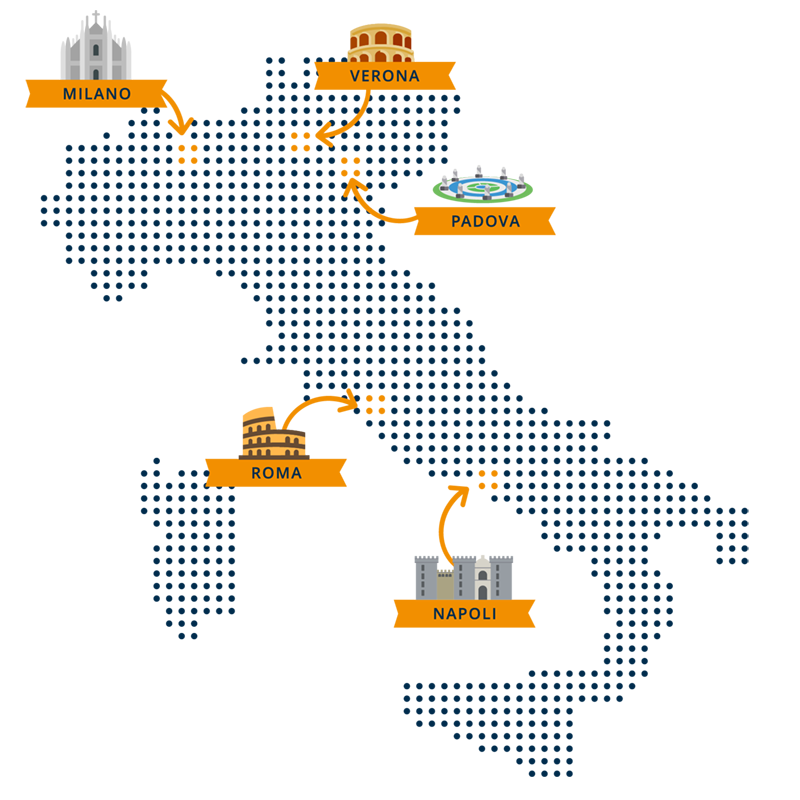
\includegraphics[width=8cm]{immagini/sedi.png}
	\caption{Sedi Sync Lab}
	\label{fig:Sedi Sync Lab}
\end{figure}
\\
Sync Lab, propone sul mercato interessanti e innovativi prodotti software, nati nel proprio laboratorio di ricerca e sviluppo. Attraverso questi prodotti, Sync Lab ha gradualmente conquistato significativamente fette di mercato nei seguenti settori: mobile, videosorveglianza e sicurezza delle infrastrutture informatiche aziendali.

%**************************************************************
\section{Metodologie utilizzate e principali prodotti}
L’azienda adotta un modello di sviluppo agile che pone le proprie basi nel metodo Scrum. Gli stakeholders, infatti, vengono costantemente coinvolti nel processo di
sviluppo del prodotto per raccogliere feedback. Gli obiettivi si possono riassumere in tre punti fondamentali:
\begin{itemize}
	\item Comprendere attentamente il contesto operativo del cliente; 
	\item Fornire al cliente un supporto mirato; 
	\item Accelerare e favorire la formazione di soluzioni. 
\end{itemize}
In base a questi principi Sync Lab raggiunge i propri obiettivi grazie a:
\begin{itemize}
	\item Consulenza; 
	\item Fornitura; 
	\item Sviluppo; 
	\item Manutenzione. \\
\end{itemize}

Nell'ambito di prodotti e innovazioni, l'azienda ne può vantare un buon numero.
Tra questi troviamo: 
\begin{itemize}
	\item \textbf{SynClinic} che è un  software integrato per la gestione delle strutture sanitarie, che permette di gestire, organizzare e monitorare tutte le fasi del percorso di cura del paziente; \\
	\begin{figure}[htbp]	
		\centering
		
\includegraphics[width=7cm]{immagini/synClinic.jpg}
		\caption{SynClinic}
		\label{fig:SynClinic}
	\end{figure}
	\\
	\item \textbf{DPS 4.0} che permette di gestire la General Data Protection Regulation(GDPR) Privacy in pochi semplici passi con una soluzione guidata per aggiornare e modificare i documenti di privacy in modo conforme agli standard di riferimento; \\
	\item \textbf{StreamLog} che permette di gestire la compliance al provvedimento del Garante per la protezione dei dati personali relativo agli Amministratori di Sistema (AdS). In particolare, permette di soddisfare requisiti fissati dal Garante; \\
	\item \textbf{StreamCrusher} che è una tecnologia che aiuta ad essere bene informati su quando bisogna prendere decisioni di business, ad identificare velocemente criticità ed a riorganizzare i processi in base a nuove esigenze; \\
	\item \textbf{Wave} che si propone come integrazione tra i mondi della Videosorveglianza e quello dei Sistemi Informativi Territoriali (GIS) abilitando il controllo totale dell'area da sorvegliare; \\
	\item \textbf{Seastream} che mette a disposizione un sistema di monitoraggio avanzato delle flotte armatoriali operative in tutto il mondo e una piattaforma integrata di servizi per gli operatori in ambito portuale. \\
\end{itemize}



%**************************************************************

             % Introduzione
% !TEX encoding = UTF-8
% !TEX TS-program = pdflatex
% !TEX root = ../tesi.tex

%**************************************************************
\chapter{Descrizione dello stage e obiettivi}
\label{cap:Descrizione dello stage e obiettivi}
%**************************************************************

\intro{In questo capitolo viene introdotto il progetto di stage e viene descritto come è stato organizzato il lavoro in azienda con gli obiettivi iniziali e le variazioni rispetto a quanto pianificato inizialmente.}\\

%**************************************************************
\section{Introduzione al progetto e scopo}
Lo scopo del progetto di stage è lo sviluppo di una piattaforma web-mobile per la gestione di eventi sportivi. Questa applicazione permette ai vari utenti di visualizzare varie attività sportive, presenti o future, così da poter partecipare premendo semplicemente su un bottone. Prima di iniziare il progetto di stage era già presente una prima versione dell'applicazione, creata da uno stagista in passato, che però non conteneva tutte le funzionalità necessarie. L'obiettivo principale è stato infatti riprendere il codice esistente, migliorarlo e completarlo con le funzionalità mancanti. È stata effettuata una fase iniziale di analisi e progettazione, basata sull’utilizzo del framework Flutter in linguaggio Dart, seguita dalla realizzazione di alcune parti dell’interfaccia mobile.
Regolarmente, ci sono stati incontri diretti con il tutor aziendale Fabio Pallaro per verificare lo stato di avanzamento, chiarire eventualmente gli obiettivi, affinare la ricerca e aggiornare il piano di lavoro.

\section{Obiettivi dello stage}
Come obiettivi è stato richiesto di:
\begin{enumerate}
	\item Realizzare le funzionalità indicate;
	\item Produrre un documento Tecnico che descriva le funzionalità realizzate;
	\item Rilasciare il codice sul repository che verrà indicato dall’azienda.\\
	
\end{enumerate}
\subsection*{Notazione}
Per gli obiettivi delle stage si farà riferimento ai requisiti secondo le seguenti notazioni:
\begin{itemize}
	\item \textit{O} per i requisiti obbligatori, vincolanti in quanto obiettivo primario richiesto dal committente;
	\item \textit{D} per i requisiti desiderabili, non vincolanti o strettamente necessari,
	ma dal riconoscibile valore aggiunto;
	\item \textit{F} per i requisiti facoltativi, rappresentanti valore aggiunto non strettamente 
	competitivo.
\end{itemize}

Le sigle precedentemente indicate saranno seguite da una coppia sequenziale di numeri, identificativo del requisito.

\subsection*{Obiettivi fissati}
Si prevede lo svolgimento dei seguenti obiettivi:
\begin{itemize}
	\item Obbligatori
	\begin{itemize}
		\item	O01: Acquisizione delle competenze sulle tematiche sopra descritte e sulle attività svolte; \\
		\item O02: Capacità di raggiungere gli obiettivi richiesti in autonomia seguendo il cronoprogramma;\\
		\item O03: Portare a termine le implementazioni previste con una percentuale di superamento pari all’80\%.\\
	\end{itemize}
	
	\item Desiderabili 
	\begin{itemize}
		\item D01: Portare a termine le implementazioni previste con una percentuale di superamento pari al 100\%.\\
	\end{itemize}
	
	\item Facoltativi
	\begin{itemize}
		\item F01:  Realizzazione di una nuova funzionalità per l'app che prevede la gestione Signin con il protcollo Oath2.\\
	\end{itemize} 
\end{itemize}

\section{Pianificazione del lavoro}
In questa sezione viene mostrato come è stato pianificato il lavoro e le variazioni apportate in seguito agli incontri regolari con il tutor aziendale Fabio Pallaro.
\subsection{Pianificazione iniziale}
Inizialmente è stata fatta una pianificazione basata su 8 settimane con una ripartizione di 40 ore per ciascuna settimana per un totale di 320 ore.
La pianificazione iniziale è la seguente:
 \begin{itemize}
	\item \textbf{Prima Settimana (40 ore)}
	\begin{itemize}
		\item Presentazione strumenti di lavoro per la condivisione del materiale di studio e per la gestione
		dell’avanzamento;
		\item Condivisione scaletta di argomenti;
		\item Ripasso del linguaggio Java SE;
		\item Ripasso concetti Web (Servlet, servizi Rest, Json ecc.).
	\end{itemize}
	\item \textbf{Seconda Settimana (40 ore)} 
	\begin{itemize}
		\item Studio principi generali di Flutter e linguaggio Dart;
		\item Studio delle best practice Flutter;
		\item Studio delle architetture per i services in Flutter.
	\end{itemize}
	\item \textbf{Terza Settimana (40 ore)} 
	\begin{itemize}
		\item Studio dei widget in Flutter;
		\item Studio del prototipo di app SportWill oggi esistente.
	\end{itemize}
	\item \textbf{Quarta Settimana (40 ore)} 
	\begin{itemize}
		\item Implementazione del login/signup con salvataggio credenziali su localStorage con aggiunta di foto ed altre info dell'utente corrente;
		\item Modifica dell'interfaccia grafica nella visualizzazione 'Elenco Uscite' con filtri di ricerca.
	\end{itemize}
	\item \textbf{Quinta Settimana (40 ore)} 
	\begin{itemize}
		\item Modifica funzionalità 'Modifica Uscita';
		\item Implementazione della funzionalità 'Inserisci mappa percorso';
		\item Implementazione della funzionalità 'Uscita in esecuzione/archiviata'.
	\end{itemize}
	\item \textbf{Sesta Settimana (40 ore)} 
	\begin{itemize}
		\item Implementazione della funzionalità 'WaitForMe' per le uscite in esecuzione.
	\end{itemize}
	\item \textbf{Settima Settimana (40 ore)} 
	\begin{itemize}
		\item Termine implementazione funzionalità 'WaitForMe'.
	\end{itemize}
	\item \textbf{Ottava Settimana (40 ore)} 
	\begin{itemize}
		\item Termine integrazioni e collaudo finale.
	\end{itemize}
\end{itemize}
\newpage
La pianificazione iniziale, in termini di quantità di ore di lavoro, è così distribuita nella \hyperref[tab:Tabella riassuntiva della pianificazione iniziale di stage]{Tabella 2.1}:

\begin{center}
\begin{table}[h!]
	
	\label{tab:Tabella riassuntiva della pianificazione iniziale di stage}
	\begin{tabularx}{\textwidth}{|c|X|}
		
		\hline
		\textbf{Durata in ore} & \textbf{Descrizione dell'attività} \\\hline
		
		\textbf{40} & \textbf{Formazione sulle tecnologie} \\	 
		\hline
		
		\textbf{80} & \textbf{Definizione architettura di riferimento e relativa documentazione} \\  \hdashline
		\multirow{3}{0cm}\\ 
		\textit{13} & 
		\textit{Studio principi generali di Flutter e linguaggio Dart} \\
		\textit{13} & 
		\textit{Studio delle best practice Flutter} \\
		\textit{14} & 
		\textit{Studio delle architetture per i services in Flutter} \\
		\textit{20} & 
		\textit{Studio dei widget in Flutter} \\
		\textit{20} & 
		\textit{Studio del prototipo di app SportWill oggi esistente} \\
		\hline
		\textbf{160} & \textbf{Implementazioni} \\ \hdashline
		\multirow{3}{0cm}\\ 
		\textit{20} & 
		\textit{Implementazione del login/signup con salvataggio credenziali su localStorage con aggiunta di foto ed altre info dell’utente corrente} \\
		\textit{20} & 
		\textit{Modifica dell’interfaccia grafica nella visualizzazione ’Elenco Uscite’ con filtri di ricerca} \\
		\textit{10} & 
		\textit{Modifica funzionalità ’Modifica Uscita’} \\
		\textit{15} & 
		\textit{Implementazione della funzionalità ’Inserisci mappa percorso’} \\
		\textit{15} & 
		\textit{Implementazione della funzionalità ’Uscita in esecuzione/archiviata’} \\
		\textit{40} & 
		\textit{Implementazione della funzionalità ’WaitForMe’ per le uscite in esecuzione.} \\
		\textit{40} & 
		\textit{Termine implementazione funzionalità ’WaitForMe’} \\
		\hline
		
		\textbf{40} & \textbf{Termine integrazioni e collaudo finale.}  \\ 
		\hline
		
		\hline
		\textbf{Totale ore: 320} &  \\\hline	
	\end{tabularx}
	\vspace{0.3cm}
	\caption{Tabella riassuntiva della pianificazione iniziale di stage}
\end{table}
\end{center}
\subsection{Variazioni}
Rispetto a quanto pianificato all'inizio sono variate le funzionalità da realizzare,in quanto quelle previste sono state suddivise con un altro stagista.
Le variazioni in particolar modo sono dalla quarta alla settima settimana e sono le seguenti:
\begin{itemize}
\item \textbf{Quarta Settimana (40 ore)} 
\begin{itemize}
	\item Configurazione iniziale;
	\item Modifica logo;
	\item Modifica dell'interfaccia grafica nella visualizzazione 'Elenco Uscite' con filtri di ricerca.
\end{itemize}
\item \textbf{Quinta Settimana (40 ore)} 
\begin{itemize}
	\item Modifica funzionalità 'Modifica Uscita' con vari fix e cambio colori;
	\item Implementazione della funzionalità 'Visualizza mappa percorso'.
\end{itemize}
\item \textbf{Sesta Settimana (40 ore)} 
\begin{itemize}
	\item Implementazione della funzionalità che permette di vedere la mappa a schermo intero;
	\item Implementazione della funzionalità che permette l'aggiornamento automatico della mappa.
\end{itemize}
\item \textbf{Settima Settimana (40 ore)} 
\begin{itemize}
	\item Modifica dell'interfaccia grafica nella visualizzazione 'Elenco Uscite' con filtri di ricerca avanzati.
\end{itemize}
\end{itemize}
La pianificazione, in termini di quantità di ore di lavoro dopo la variazione è così distribuita nella \hyperref[tab:Tabella riassuntiva della pianificazione di stage con variazioni]{Tabella 2.2}:
\begin{center}
	\begin{table}[h!]
		
		\label{tab:Tabella riassuntiva della pianificazione di stage con variazioni}
		\begin{tabularx}{\textwidth}{|c|X|}
			
			\hline
			\textbf{Durata in ore} & \textbf{Descrizione dell'attività} \\\hline
			
			\textbf{40} & \textbf{Formazione sulle tecnologie} \\	 
			\hline
			
			\textbf{80} & \textbf{Definizione architettura di riferimento e relativa documentazione} \\  \hdashline
			\multirow{3}{0cm}\\ 
			\textit{13} & 
			\textit{Studio principi generali di Flutter e linguaggio Dart} \\
			\textit{13} & 
			\textit{Studio delle best practice Flutter} \\
			\textit{14} & 
			\textit{Studio delle architetture per i services in Flutter} \\
			\textit{20} & 
			\textit{Studio dei widget in Flutter} \\
			\textit{20} & 
			\textit{Studio del prototipo di app SportWill oggi esistente} \\
			\hline
			\textbf{160} & \textbf{Implementazioni} \\ \hdashline
			\multirow{3}{0cm}\\
			\textit{15} & 
			\textit{Configurazione iniziale} \\ 
			\textit{5} & 
			\textit{Modifica logo} \\ 
			\textit{20} & 
			\textit{Modifica dell’interfaccia grafica nella visualizzazione ’Elenco Uscite’ con filtri di ricerca} \\
			\textit{10} & 
			\textit{Modifica funzionalità 'Modifica Uscita' con vari fix e cambio colori} \\
			\textit{30} & 
			\textit{Implementazione della funzionalità 'Visualizza mappa percorso'} \\
			\textit{10} & 
			\textit{Implementazione della funzionalità che permette di vedere la mappa a schermo intero} \\
			\textit{30} & 
			\textit{Implementazione della funzionalità che permette l'aggiornamento automatico della mappa.} \\
			\textit{40} & 
			\textit{Modifica dell'interfaccia grafica nella visualizzazione 'Elenco Uscite' con filtri di ricerca avanzati.} \\
			\hline
			\textbf{40} & \textbf{Termine integrazioni e collaudo finale.}  \\ 
			\hline
			
			\hline
			\textbf{Totale ore: 320} &  \\\hline	
		\end{tabularx}
		\vspace{0.3cm}
		\caption{Tabella riassuntiva della pianificazione di stage con variazioni}
	\end{table}
\end{center}
\newpage
\section{Strumenti di comunicazione per lo svolgimento del lavoro}
Per supportare lo svolgimento del lavoro sono stati usati i seguenti strumenti di comunicazione:
\begin{itemize}
	\item \textbf{Trello} (vedi Figura 2.1) che mi ha permesso di organizzare e di gestire il progetto tramite la creazione di una bacheca condivisibile;
	\begin{figure}[htbp]	
		\centering
		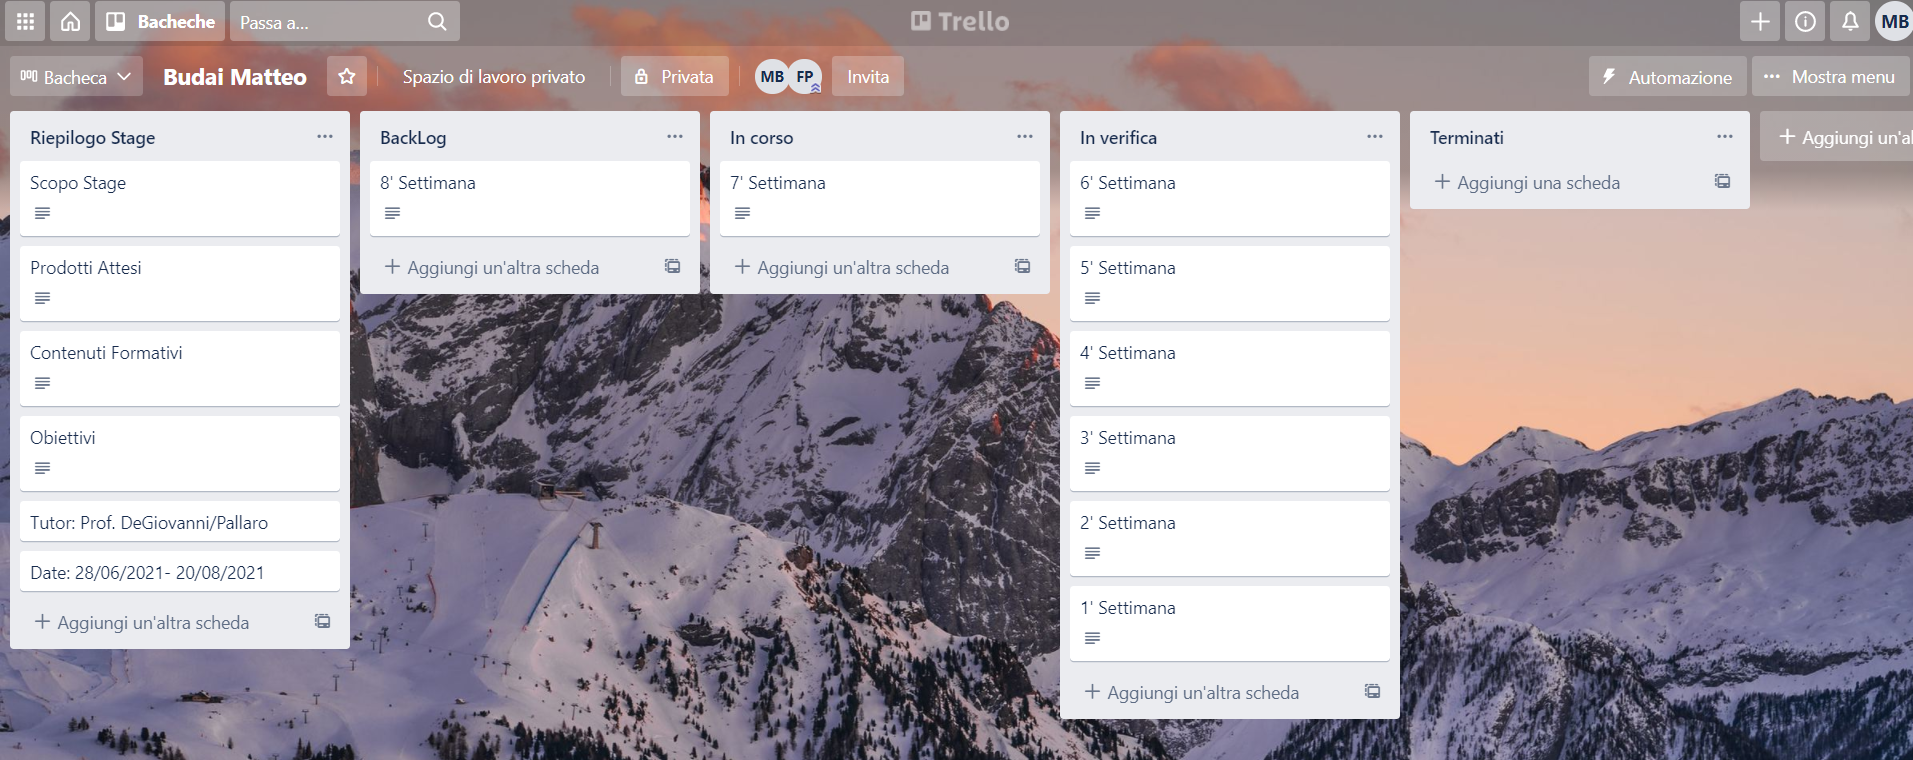
\includegraphics[width=12cm]{immagini/trello.png}
		\caption{Trello}
		\label{fig:Trello}
	\end{figure}
	\item \textbf{Google sheets} (vedi Figura 2.2) in cui venivano riportate ogni giorno le attività che si andavano a svolgere. Veniva segnalato con una spunta se l'attività era corretta oppure nella colonna aggiustamenti veniva spiegato in che modo correggere l'attività o cosa svolgere;
	\begin{figure}[htbp]	
		\centering
		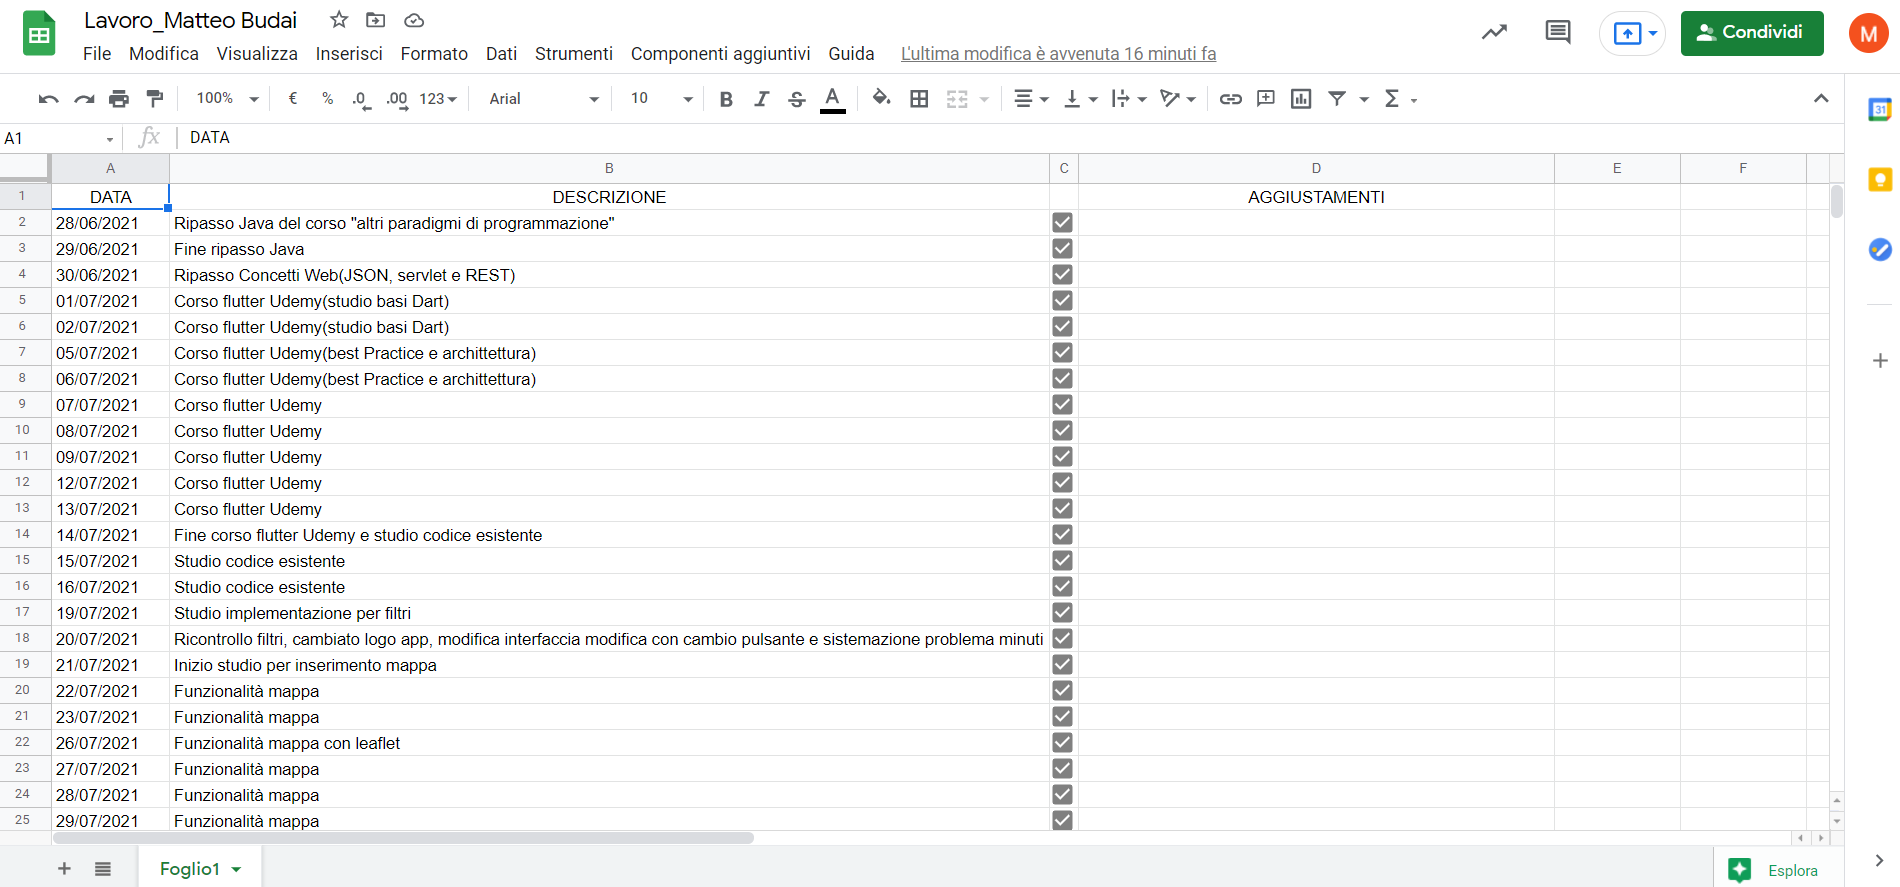
\includegraphics[width=12cm]{immagini/googlesheet.png}
		\caption{Google sheets}
		\label{fig:Google sheets}
	\end{figure}
	\item \textbf{Discord} che mi ha permesso di interfacciarmi direttamente
	con il tutor aziendale Fabio Pallaro e con tutti i membri di SyncLab sfruttando più canali di comunicazione vocali e testuali, divisi per argomenti.
\end{itemize}
	


             % Processi
% !TEX encoding = UTF-8
% !TEX TS-program = pdflatex
% !TEX root = ../tesi.tex

%**************************************************************
\chapter{Framework Flutter e linguaggio Dart}
\label{cap:Framework Flutter e linguaggio Dart}
%**************************************************************

\intro{In questo capitolo, viene introdotto come un'applicazione mobile può essere sviluppata per poi concentrarsi su Flutter e tutte le sue componenti. Infine saranno mostrate come esempio alcune piccole applicazioni realizzate per imparare a utilizzare il framework Flutter.}\\

%**************************************************************
\section{Sviluppo applicazioni mobile}
Nel quotidiano, non solo in Italia ma in tutto il mondo, l'uso dello smartphone \cite{statistiche} è in costante aumento. \\
Mentre fino a qualche anno fa il cellulare veniva usato solo per telefonare o mandare qualche messaggio, oggi lo smartphone viene utilizzato in qualsiasi ambito: lavoro, comunicare, divertirsi, video, musica o svago. \\
Ormai nei cellulari sono presenti applicazioni per qualsiasi esigenza ed è proprio per questo che chi sviluppa applicazioni ha dovuto considerare lo sviluppo per mobile come fattore primario.\\
	\begin{figure}[htbp]	
	\centering
	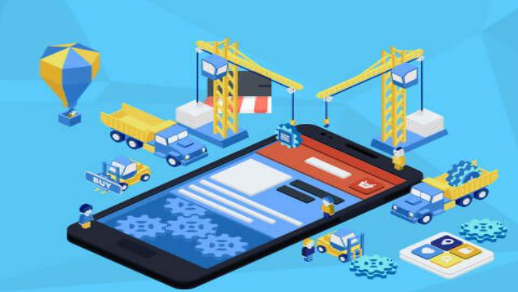
\includegraphics[width=10cm]{immagini/sviluppoapp.png}
	\caption{Sviluppo applicazioni mobile}
	\label{fig:Sviluppo applicazioni mobile}
\end{figure}
\\
Esistono quattro diversi approcci di implementazione: 
\begin{itemize}
	\item App native; 
	\item Web app; 
	\item App Ibride Web View Wrapper; 
	\item App Ibride Compile to Native.
\end{itemize}
\cite{sviluppo,differenza,apptonative}

\subsection{App native}
Il metodo nativo \cite{differenza,apptonative} da la possibilità all'applicazione di integrarsi con la parte hardware del dispositivo, sfruttando così tutte le funzionalità del sistema operativo. \\
Le app native vengono realizzate utilizzando gli strumenti di sviluppo software e la documentazione fornita dai produttori del sistema operativo per il quale si ha l'intenzione di sviluppare.\\
Questo metodo è scelto sopratutto degli sviluppatori attenti alle prestazioni e alle performance dell'applicazione.\\
I vantaggi principali di sviluppare App native sono:
\begin{itemize}
	\item Maggiore velocità, affidabilità e reattività;
	\item Accesso diretto alla parte hardware e al software installato nel device; 
	\item Notifiche dirette;
	\item Funzionamento offline.
\end{itemize}
Attualmente i sistemi operativi più utilizzati sono:
\begin{itemize}
	\item Android; 
	\item iOS; 
	\item Windows Phone.\\
\end{itemize}
\cite{sviluppo}

\subsubsection{Android}
\begin{figure}[htbp]	
	\centering
	
\includegraphics[width=1cm]{immagini/logoandroid.png}
	\caption{Logo Android}
	\label{fig:Logo Android}
\end{figure}
 Android è il sistema operativo più utilizzato e diffuso. È stato sviluppato da Google ed è stato scelto da multinazionali importanti come Samsung, Huawei e Amazon per il funzionamento dei loro dispositivi.\\
 Il linguaggio per sviluppare un'applicazione Android è Java. Negli ultimi anni è nato anche Kotlin, che è un altro linguaggio ufficiale per la progettazione di applicazioni Android più moderno, meno complesso ma performante e compatibile con l'ambiente Android quanto Java.\\
 \newpage

 \subsubsection{iOS}
 \begin{figure}[htbp]	
 	\centering
 	
\includegraphics[width=1cm]{immagini/logoios.jpg}
 	\caption{Logo iOS}
 	\label{fig:Logo iOS}
 \end{figure}
 iOS è il sistema operativo sviluppato da Apple per dispositivi iPhone, iPod touch e iPad.\\
 Per un lungo periodo il linguaggio per sviluppare un'applicazione iOS è stato Objective-C che deriva da C e C++. \\
 Per aumentare la produttività, Apple ha lanciato un linguaggio di più alto livello ovvero Swift. Swift è veloce, leggibile e poco prolisso. Nonostante ciò, Objective-C viene ancora preferito quando si sta lavorando più a basso livello.\\

 \subsubsection{Windows Phone}
 \begin{figure}[htbp]	
 	\centering
 	
\includegraphics[width=3cm]{immagini/logowindowsphone.png}
 	\caption{Logo Windows Phone}
 	\label{fig:Logo Windows Phone}
 \end{figure}
Windows Phone è il sistema operativo sviluppato da Microsoft.\\
Il linguaggio utilizzato per sviluppare un'applicazione Windows Phone è C\#, che è un linguaggio semi-compilato orientato agli oggetti.\\
Con Android e iOS in ambito mobile non c'è paragone. Invece per quanto riguarda sistemi desktop, Windows risulta una delle migliori.\\
 
\subsection{Web app}
Una web app \cite{differenza,apptonative} è un'applicazione che funziona come un sito web adattandosi al dispositivo utilizzato.\\
Queste applicazioni non necessitano di essere installate sugli smartphone e quindi non andranno ad aumentare la memoria utilizzata nel dispositivo.\\
 Inoltre non possono essere pubblicate sugli Store e quindi non godono di un enorme visibilità.\\
I principali framework e librerie per creare una web app sono:
\begin{itemize}
	\item Angular; 
	\item PolymerJS; 
	\item React.
\end{itemize}
I vantaggi di sviluppare una web app sono:
\begin{itemize}
	\item Scrittura con Markup HTML;
	\item Non essendo pubblicate sul Market non devono essere sottoposte al processo di approvazione; 
	\item Minor tempo di sviluppo.
\end{itemize}

\newpage

\subsection{App Ibride Web View Wrapper}
Questo tipo di metodo \cite{differenza,apptonative} permette di creare applicazioni senza alcuna conversione del codice in base al sistema operativo.\\
 In pratica l'applicazione rileva inizialmente il sistema operativo utilizzato e successivamente imita l'aspetto dell'interfaccia utente, utilizzando CSS, Sass...\\
Le piattaforme più usate sono:
\begin{itemize}
\item Ionic; 
\item Apache Cordova; 
\item PhoneGap.
\end{itemize}
I vantaggi principali di Ionic e delle App Ibride Web View Wrapper sono:
\begin{itemize}
	\item Riutilizzo facile del codice; 
	\item Ionic utilizza JavaScript e fornisce un supporto per Angular;
	\item Addatamento automatico in base alla piattaforma; 
\end{itemize}
Lo svantaggio principale di questo tipo di applicazioni sta in termini di velocità di calcolo e questo comporterà prestazioni inferiori alle applicazione compilate in nativo.\\

\subsection{App Ibride Compile to Native}
Le applicazioni ibride che compilano in nativo \cite{apptonative} utilizzano un unico linguaggio di programmazione per la scrittura del codice.\\
 Una volta compilato, i componenti dell'interfaccia utente del codice vengono convertiti nei componenti dell'interfaccia utente nativi senza bisogno di configurazioni particolari.\\
Le principali piattaforme utilizzate per compilare in nativo sono:
\begin{itemize}
	\item React Native; 
	\item NativeScript; 
	\item Xamarin; 
	\item Flutter.
\end{itemize}
I vantaggi principali di utilizzare piattaforme che compilano in nativo sono:
\begin{itemize}
	\item Anche se minore delle App Ibride Web View Wrapper hanno un elevata riutilizzabilità del codice; 
	\item Elevato numero di librerie utilizzabili;  
	\item Compilando in nativo offrono prestazioni elevate.
\end{itemize}
\newpage
\section{Flutter}
\begin{figure}[htbp]	
	\centering
	
\includegraphics[width=5cm]{immagini/flutterlogo.jpg}
	\caption{Logo Flutter}
	\label{fig:Logo Flutter}
\end{figure}
Flutter \cite{flutter,flutterprogramma,fluttermobile} è un framework nato abbastanza di recente per lo sviluppo di applicazioni per diverse piattaforme.\\
È stato ideato da Google come progetto open source e pubblicato ufficialmente per la prima volta a dicembre del 2018 nella versione 1.0 all'evento Flutter Live.\\
Il 3 marzo 2021 è stata rilasciata la versione 2.0 che consente agli sviluppatori di generare in maniera stabile applicazioni multipiattaforma.\\
Flutter offre una vasta serie di librerie di elementi di interfaccia utente e combina la facilità di sviluppo con prestazioni simili alle prestazioni native, mantenendo una corretta distinzione visiva tra le diverse piattaforme senza che il programmatore debba prestare particolari attenzioni.\\
Viene utilizzato sopratutto per applicazioni Android e iOS e funziona come una vera applicazione nativa.\\
Utilizzando lo stesso codebase è possibile creare l'applicazione per diverse piattaforme.\\
Il linguaggio di programmazione di Flutter è Dart, sviluppato anche esso da Google, ed è stato pensato per sostituire JavaScript.\\
Flutter è completamente gratuito e come possiamo vedere dalla figura sottostante, già nell'ultimo anno la sua popolarità e il suo utilizzo è cresciuto notevolmente.\\
\begin{figure}[htbp]	
	\centering
	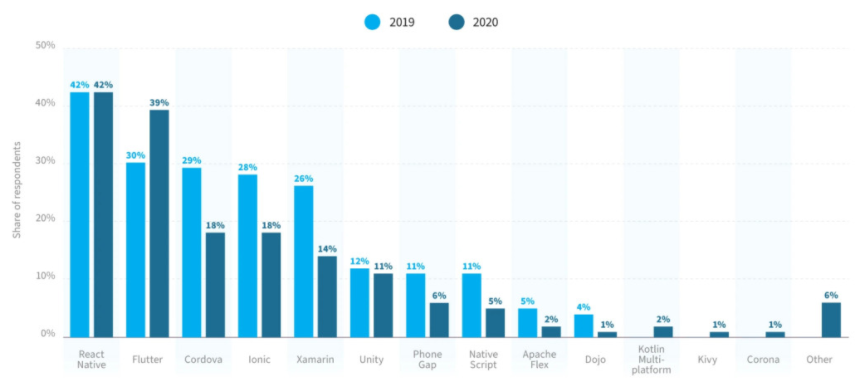
\includegraphics[width=13cm]{immagini/statisticheflutter.png}
	\caption{Statistiche dei programmatori che usano Flutter per sviluppare app mobile}
	\label{fig:Statistiche dei programmatori che usano Flutter per sviluppare app mobile}
\end{figure}
\newpage
Anche se molto recente, nel Google Play Store possiamo contare oltre 50000 applicazioni Flutter.\\
I vantaggi di utilizzare Flutter sono:
\begin{itemize}
	\item Un codebase per tutte le piattaforme; 
	\item Utilizzo di \hyperref[sec:Dart]{Dart} che è un linguaggio facile da apprendere;  
	\item È più facile sviluppare applicazioni con Flutter che quindi entrano sul mercato più in fretta;
	\item Si basa sul principio \textit{'Tutto è un Widget'} che sarà spiegato nella \hyperref[sec:Widget]{sezione Widget};
	\item Basso consumo di risorse;
	\item Esecuzione performante delle app native su smartphone;
	\item Ottima interfaccia utente che può essere anche personalizzata;
	\item L’hot reload permette di vedere le modifiche in tempo reale accelerando lo sviluppo.\\
\end{itemize}
Invece tra gli svantaggi possiamo citare che:
\begin{itemize}
	\item Dart è un linguaggio nuovo e quindi non è molto diffuso; 
	\item Essendo nuovo mancano librerie di terze parti che facilitano lo sviluppo;  
	\item Vengono create app di grandi dimensioni rispetto agli altri framework o anche a Java stesso.\\
\end{itemize}
\subsection{Dart}
\label{sec:Dart}
Dart \cite{dart,dartstoria} è un linguaggio di programmazione sviluppato da Google e presentato per la prima volta il 10 ottobre del 2011 alla conferenza 'GOTO Aarhus 2011'.\\
Lo scopo principale è quello di sostituire JavaScript per lo sviluppo delle applicazioni.\\
Dart costituisce la base di Flutter e inoltre supporta molte attività di sviluppo di base come la formattazione, l'analisi, il test del codice...\\
Dart \cite{dartover} è type-safe. Inoltre i valori in Dart non possono essere \textit{null} tranne nei casi in cui viene indicato che questi valori possono esserlo, così da evitare possibili errori nel codice.\\
Dart ha un vasto numero di librerie di base e di pacchetti per le API aggiuntive.\\
Permette di scrivere programmi attraverso due distinte piattaforme: 
\begin{itemize}
	\item Dart Native: per le applicazioni sviluppate per dispositivi mobili e desktop. Include sia una macchina virtuale Dart con compilazione JIT (just-in-time), ovvero viene compilato durante l'esecuzione del programma e facilita l'hot reload, sia un compilatore AOT (Ahead-of-Time) per la produzione di codice macchina, ovvero  viene compilato prima dell'esecuzione, tipicamente durante l'installazione del programma così migliora le prestazioni diminuendo i tempi di avvio e evitando la fase di compilazione durante l'esecuzione del programma;  
	\item Dart Web: per le applicazioni destinate al Web. Include sia un compilatore del tempo di sviluppo (dartdevc) che consente di eseguire il debug dell'applicazione nel browser Chrome e vedere le modifiche quasi immediatamente, che un compilatore del tempo di produzione (dart2js) che fornisce suggerimenti per migliorare il codice Dart e rimuovere il codice inutilizzato. Entrambi i compilatori traducono Dart in JavaScript.\\
\end{itemize}

\subsection{Componenti}
Flutter è formato da un'architettura a strati \cite{flutterdettagli, flutterd} e i suoi tre strati fondamentali sono:
\begin{itemize}
	\item Framework; 
	\item Engine;  
	\item Embedder.\\
\end{itemize}
\begin{figure}[htbp]	
	\centering
	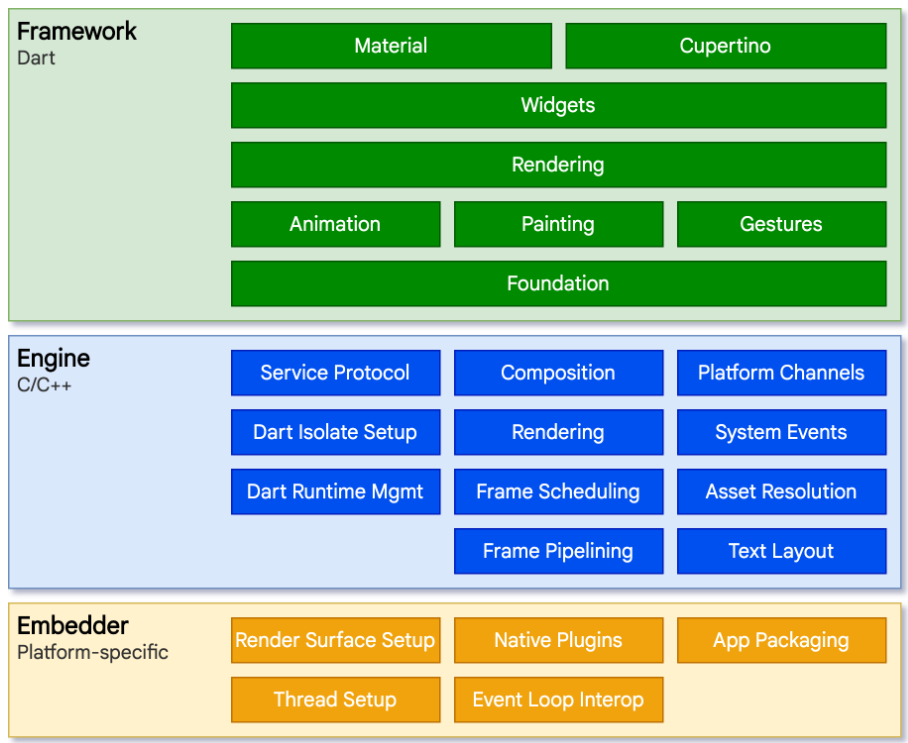
\includegraphics[width=13cm]{immagini/composizione.png}
	\caption{Architettura a strati di Flutter}
	\label{fig:Architettura a strati di Flutter}
\end{figure}

\newpage

\subsubsection{Embedder}
Embedder è il livello più basso dell'architettura.\\
Il linguaggio utilizzato è definito in base alla piattaforma e attualmente può essere: Java e C++ per Android, Objective-C/Objective-C++ per iOS e macOS e C++ per Windows e Linux.\\
Ha lo scopo di legare il rendering della schermata nativa, la gestione degli eventi e altri elementi.\\
Per fare ciò lo strato Embedder interagisce con lo strato Engine tramite delle API C/C++.\\
Inoltre lo strato Embedder è composta da una Shell che ospita anche la Dart VM.		\\
Ogni Shell è specifica per ogni piattaforma e offre un accesso alle API native della piattaforma in questione.

\subsubsection{Engine}
Engine è lo strato intermedio dell'architettura.\\
Il linguaggio utilizzato è principalmente il C++ e il C per rendere più veloci ed efficienti le applicazioni realizzate in Flutter.\\
Contiene componenti di basso livello essenziali per il funzionamento del framework.\\
All'interno troviamo il motore grafico \textit{Skia}, una libreria grafica 2D open source scritta in C++ creata da Google, e le shell a cui è possibile accedervi tramite le API esposte dalla libreria \textit{dart:ui}.

\subsubsection{Framework}
È lo strato principale dell'architettura.\\
Il linguaggio utilizzato è \hyperref[sec:Dart]{Dart}.\\
All'interno sono presenti classi fondamentali di base e servizi di base come le animazioni.\\
Inoltre è presente il Rendering che permette di gestire il layout attraverso un albero di oggetti che viene visualizzato
a schermo e che si aggiorna automaticamente.\\
Sempre all'interno di questo strato sono presenti i Widget e le due librerie: Material e Cupertino.

\newpage

\subsection{Librerie Material e Cupertino}
Le due principali librerie di Flutter sono Material e Cupertino. \cite{flutterd}\\
\begin{figure}[htbp]	
	\centering
	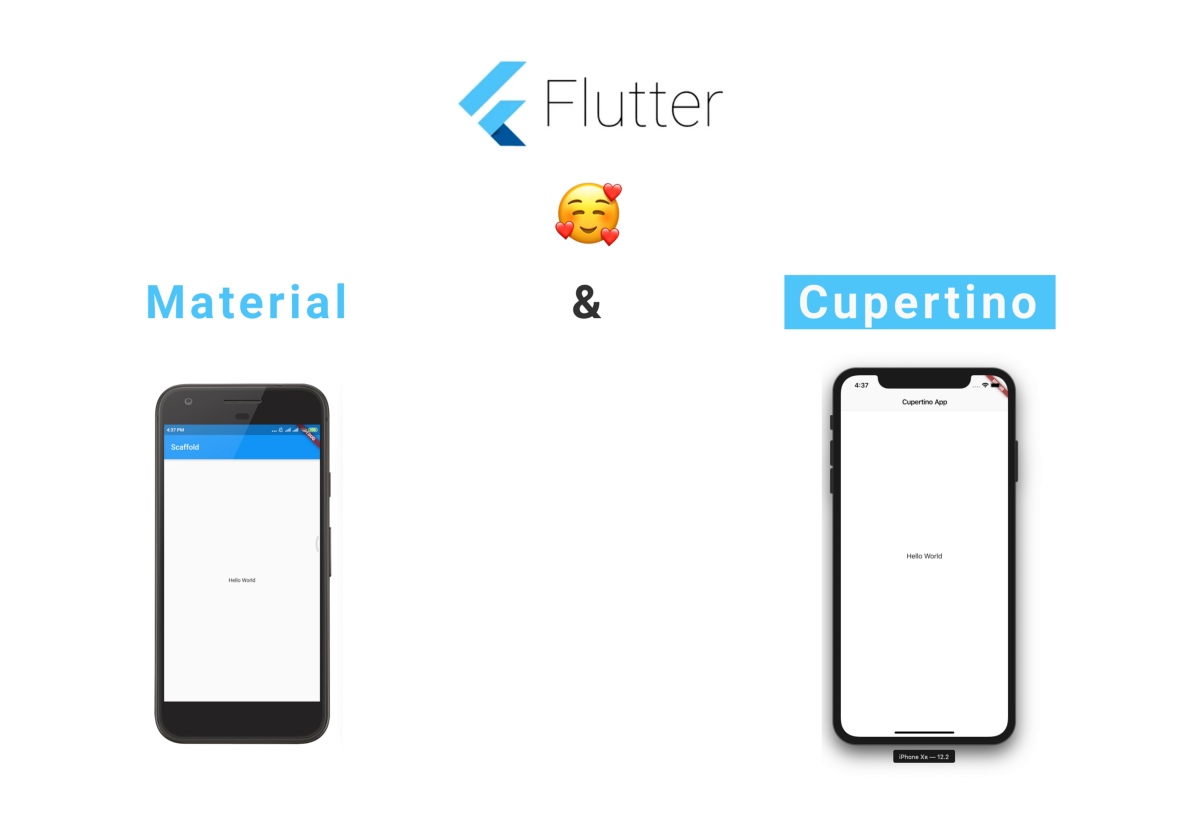
\includegraphics[width=14cm]{immagini/librerieCM.png}
	\caption{Librerie Material e Cupertino}
	\label{fig:Librerie Material e Cupertino}
\end{figure}
\\
All'interno di Flutter è possibile capire su che piattaforma si sta eseguendo l'applicazione attraverso \textit{'Platform.isIOS'}.\\
 Se ritornerà un valore booleano uguale a \textit{true} significa che saremo su iOS altrimenti saremo su Android.\\
La libreria Cupertino permette di implementare un design specifico per le applicazioni iOS.\\
A differenza della Cupertino la libreria Material permette di implementare un design specifico per le applicazioni Android.

\subsection{Widget}
\label{sec:Widget}
Flutter è basato sul principio \textit{'Tutto è un widget'} in quanto l'interfaccia di un programma è composta da diversi widget nidificati.\\
Ogni widget può essere del testo o un pulsante o un qualsiasi altro elemento grafico che contiene varie caratteristiche.\\
Tutti questi widget possono influenzare altri widget nella costruzione dell'applicazione.\\
Il vantaggio principale di questa struttura a widget consiste nella flessibilità, invece lo svantaggio di adottare questa strategia sta nel fatto che tutti i widget sono situati nel codice sorgente del programma e pertanto risulteranno fortemente nidificati.
\newpage
Il framework contiene due classi principali di widget: \cite{state, flutterd}
\begin{itemize}
	\item Stateless widget;   
	\item Stateful widget.
\end{itemize}

\begin{figure}[htbp]	
	\centering
	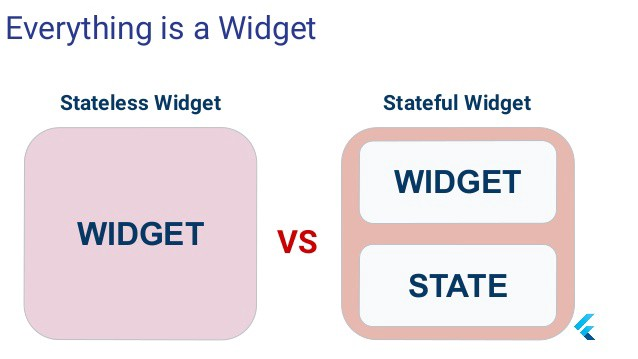
\includegraphics[width=12cm]{immagini/state.jpeg}
	\caption{Stateless widget e Stateful widget}
	\label{fig:Stateless widget e Stateful widget}
\end{figure}
\subsubsection{Stateless widget}
Gli stateless widget non hanno uno stato mutabile e quindi non cambieranno nel tempo, neanche in seguito a comportamenti effettuati dall'utente.\\
Alcuni esempi di questi widget sono: Text, Row, Column e Container.\\
Per creare uno stateless widget bisogna estendere la classe \textit{SteatelessWidget} che richiede l'override del metodo \textit{build()}.\\
Questo metodo viene invocato la prima volta per costruire l'albero dei widget e poi ogni volta che le loro dipendenze cambiano.\\
Si può usare uno stateless widget solamente quando i campi dei widget non cambiano nel tempo neanche dopo azioni dell'utente.\\
Negli altri casi sarà da utilizzare uno stateful widget.

\subsubsection{Stateful widget}
Gli stateful widget sono dinamici e mutano nel tempo in base all'interazione dell'utente o in base ad altri fattori.\\
Alcuni esempi di questi widget sono: Image, Form e Checkbox.\\
Per creare uno stateful widget bisogna estendere la classe \textit{SteatefulWidget}.\\
Come si intuisce dal nome dipendono dallo stato dell'oggetto.\\
Infatti ogni volta che si vuole modificare lo stato di un qualsiasi oggetto bisogna chiamare il metodo \textit{setState()} segnalando così al framework di aggiornare l'interfaccia utente chiamando il metodo \textit{build} e tenendo in considerazione i nuovi stati degli oggetti assegnati nel metodo appena descritto. \\
Dobbiamo quindi creare uno stateful widget quando il widget potrebbe cambiare durante il suo ciclo di vita. 

\newpage

\subsubsection{Principali Widget}
Di seguito saranno spiegati brevemente i widget più comuni e utilizzati in Flutter.

\paragraph{Scaffold}
Il widget Scaffold \cite{scaffold} implementa la struttura del layout visivo.\\
Contiene principalmente 5 elementi:
\begin{itemize}
	\item \textbf{appBar} che viene descritta in seguito;   
	\item \textbf{body} che rappresenta il corpo situato sotto l'Appbar;
	\item \textbf{floatingActionButton} che è un bottone che è situato di default in basso a destra;   
	\item \textbf{drawer} che è un menù laterale visibile dall'utente scorrendo da sinistra a destra o viceversa. All'interno di questo menù sono presenti altri widget che permettono di effettuare diverse azioni;
	\item \textbf{bottomNavigationBar} che permette di gestire un menù nella parte inferiore dell'applicazione.
\end{itemize}

\begin{figure}[htbp]	
	\centering
	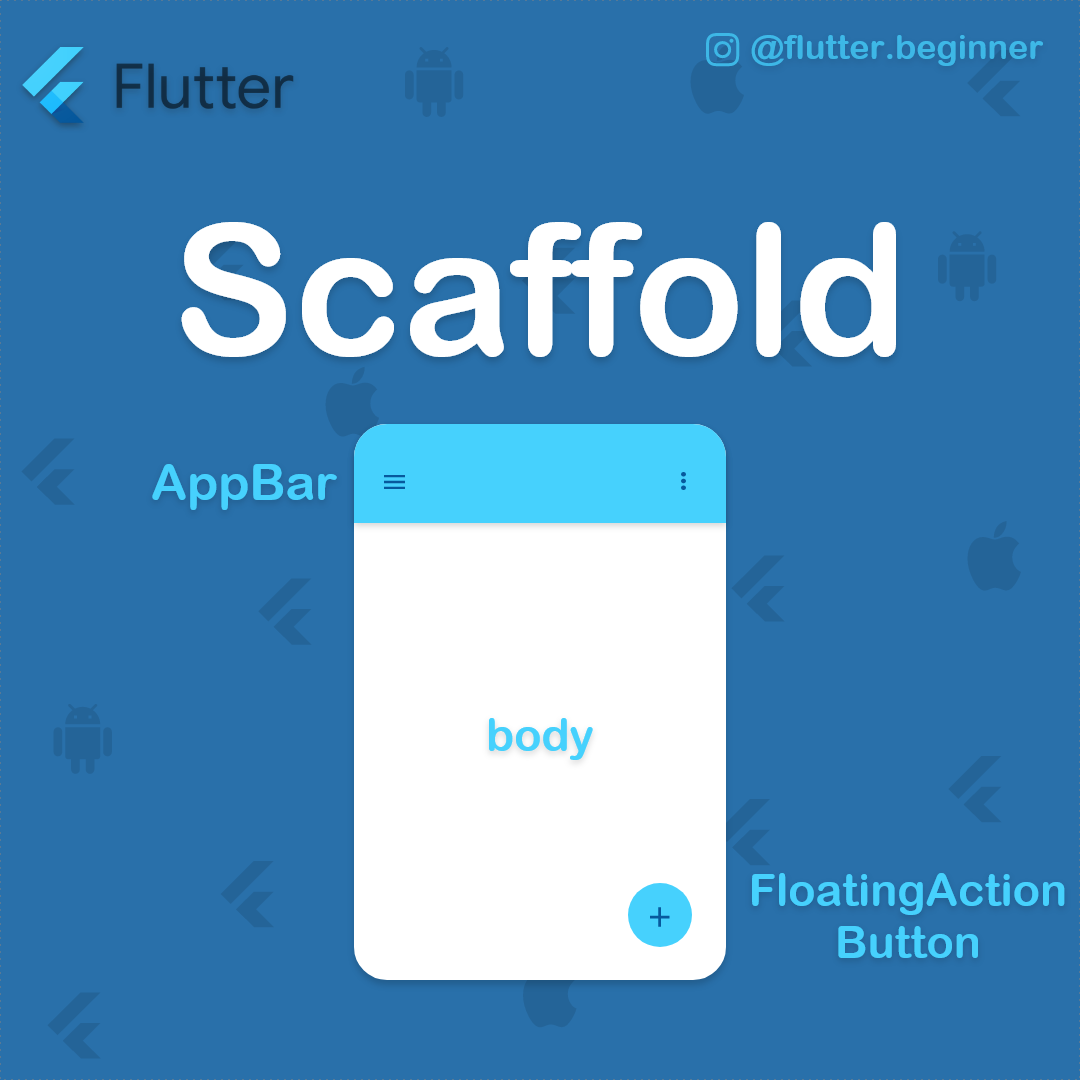
\includegraphics[width=8cm]{immagini/scaffold.png}
	\caption{Scaffold widget}
	\label{fig:Scaffold widget}
\end{figure}

\newpage

\paragraph{AppBar}
L'AppBar viene gestita da Scaffold ed è solitamente situata nella parte superiore dell'applicazione. Espone solitamente altri widget che permettono di eseguire una o più azioni.\\
AppBar ha diversi elementi grafici come elevazione e titolo.
\begin{figure}[htbp]	
	\centering
	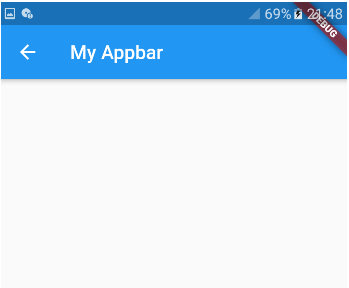
\includegraphics[width=8cm]{immagini/appbar.png}
	\caption{Appbar widget}
	\label{fig:Appbar widget}
\end{figure}

\paragraph{Row, Column}
Il widget Row permette di creare una famiglia di widget in una riga orizzontale invece il widget Column permette di creare sempre una famiglia di widget ma in verticale.\\
Entrambi non sono scorrevoli quindi nel caso si abbia bisogno di una famiglia di widget scorrevoli bisogna utilizzare il widget \textit{ListView}.
\begin{figure}[htbp]	
	\centering
	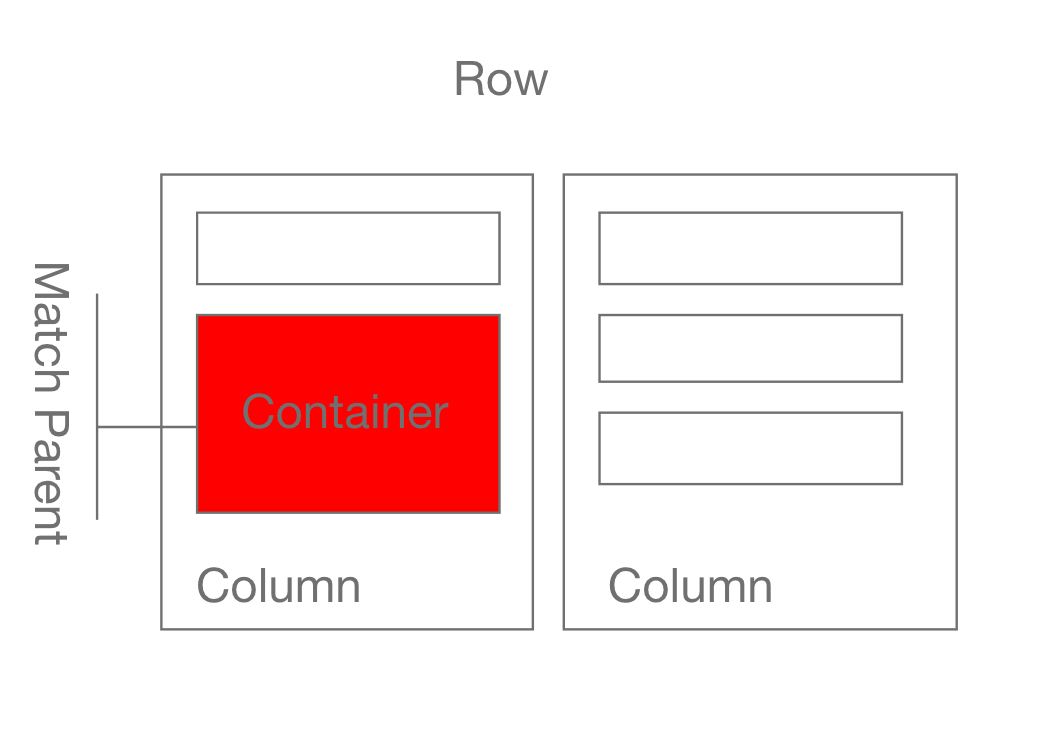
\includegraphics[width=10cm]{immagini/rowcolumn.png}
	\caption{Row e Column widget}
	\label{fig:Row e Column widget}
\end{figure}

\newpage

\paragraph{Container}
Il widget Container funge da contenitore all'interno dell'applicazione e può racchiudere altri widget.\\
Ha un margine, un bordo e un padding di default che possono essere modificati.\\
Oltre a questi elementi, questo widget contiene altri elementi che permettono di decorare la sua area di competenza.
\begin{figure}[htbp]	
	\centering
	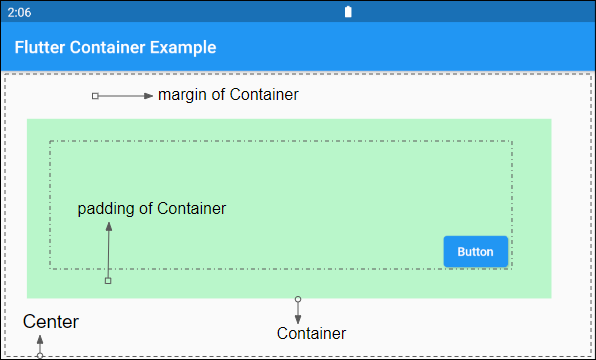
\includegraphics[width=8cm]{immagini/container.png}
	\caption{Container widget}
	\label{fig:Container widget}
\end{figure}

\paragraph{Text}
Il widget Text consente di creare una porzione di testo all'interno dell'applicazione che può essere decorata in base alle diverse esigenze.
\begin{figure}[htbp]	
	\centering
	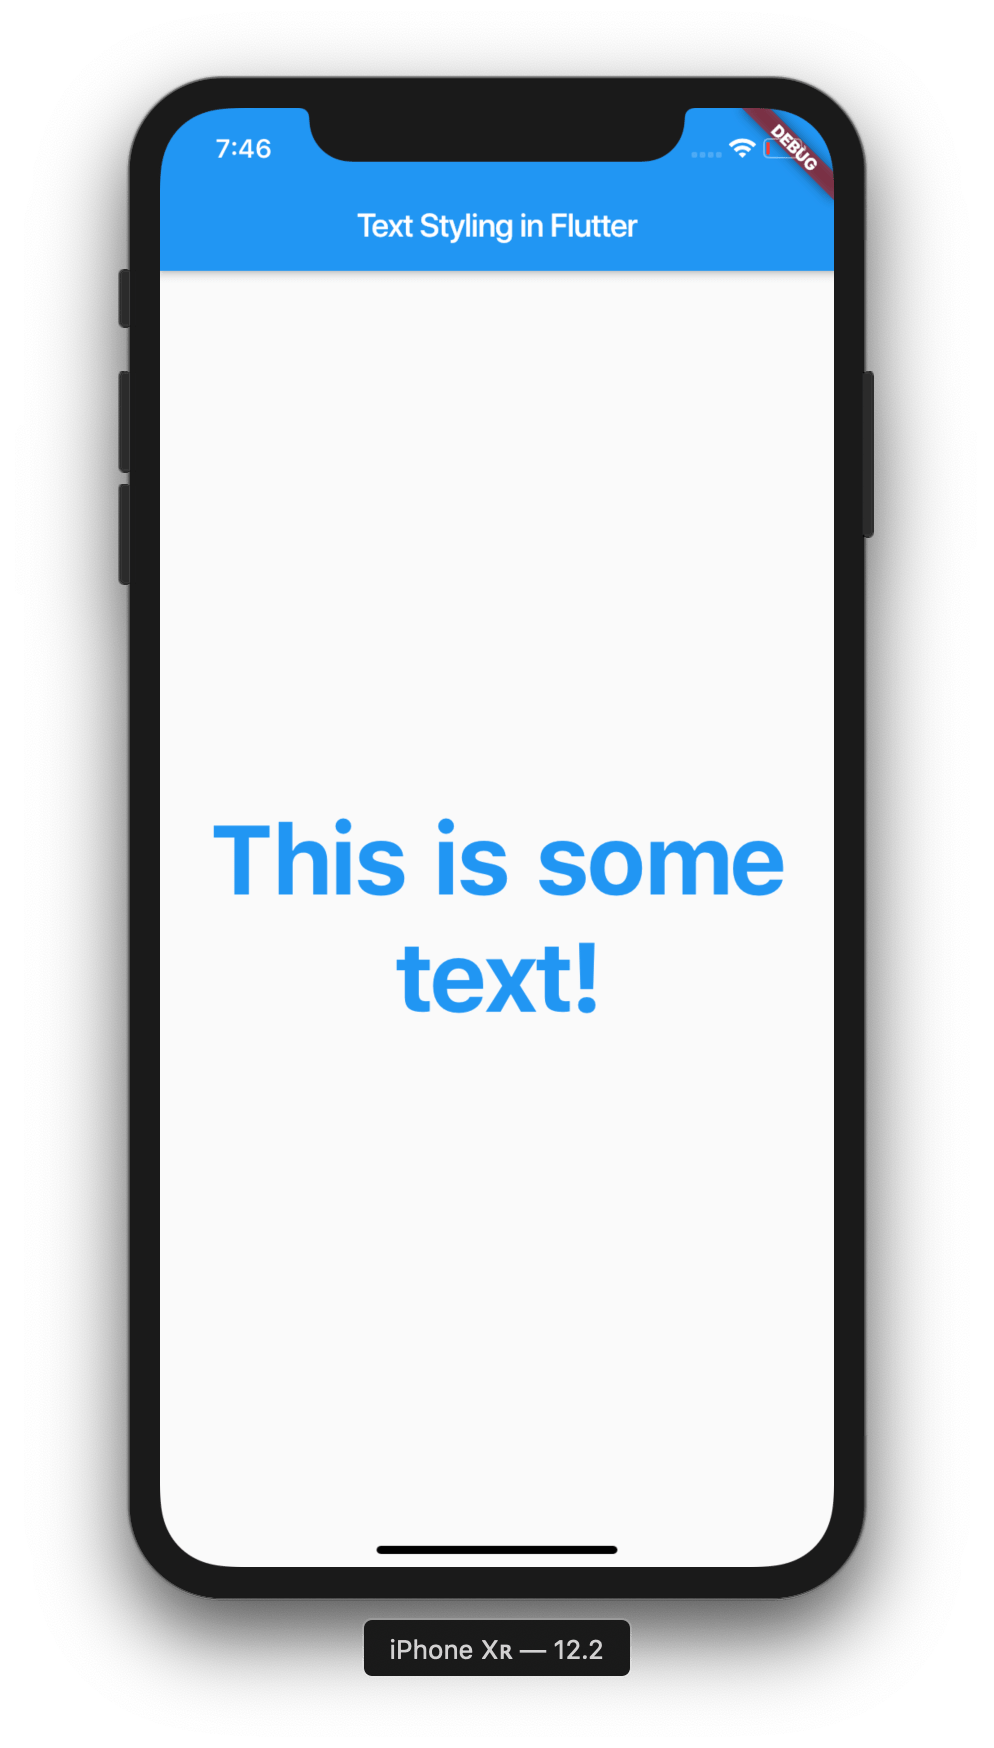
\includegraphics[width=5cm]{immagini/text.png}
	\caption{Text widget}
	\label{fig:Text widget}
\end{figure}

\paragraph{Image}
Consente di impostare all'interno dell'applicazione un'immagine.\\
Ci sono vari formati disponibili ovvero JPEG, PNG, GIF.\\
I modi per ottenere l'immagine all'interno dell'applicazione sono:
\begin{itemize}
	\item \textbf{new Image} che permette di ottenere un'immagine da un  ImageProvider(utilizza imageCache globale per memorizzare nella cache le immagini);   
	\item \textbf{new Image.asset} che permette di ottenere un'immagine da un AssetBundle(una raccolta di risorse utilizzate dall'applicazione) utilizzando una chiave;
	\item \textbf{new Image.network} che permette di ottenere un'immagine da un URL;   
	\item \textbf{new Image.file} che permette di ottenere un'immagine da un File;
	\item \textbf{new Image.memory} che permette di ottenere un'immagine da un Uint8List.
\end{itemize}

\paragraph{Icon}
Il widget Icon permette di inserire icone all'interno dell'applicazione.\\
Le icone sono quadrate e non sono interattive.
\begin{figure}[htbp]	
	\centering
	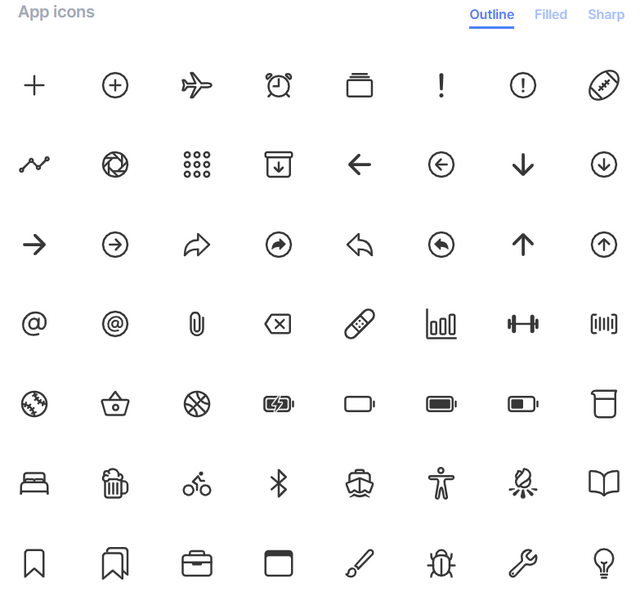
\includegraphics[width=5cm]{immagini/icon.png}
	\caption{Icon widget}
	\label{fig:Icon widget}
\end{figure}

\paragraph{ElevatedButton}
Il widget ElevatedButton permette di inserire un bottone con uno stile di default all'interno dell'applicazione.\\
Contiene l'elemento \textit{onPressed} che permette di eseguire operazioni quando il bottone viene premuto. Nel caso onPressed venga impostato uguale a \textit{null} il bottone sarà disabilitato.
\begin{figure}[htbp]	
	\centering
	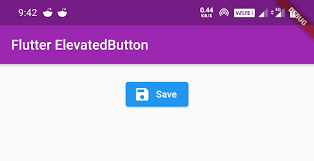
\includegraphics[width=8cm]{immagini/button.png}
	\caption{ElevatedButton widget}
	\label{fig:ElevatedButton widget}
\end{figure}

\newpage

\subsection{Esempi piccole applicazioni realizzate}
Di seguito verranno mostrate alcune applicazioni realizzate seguendo un corso su Udemy \cite{corso} per imparare a usare il framework Flutter.

\subsubsection{Applicazione base}
Dopo aver effettuato la giusta configurazione e scaricato tutto il necessario, per creare la prima applicazione di base messa a disposizione da Flutter basterà digitare sul terminale il comando: \textit{flutter create "nome\_applicazione"}.\\
Questo ci permette di creare la nostra prima applicazione base come esposto nella figura sottostante.\\

\begin{figure}[htbp]	
	\centering
	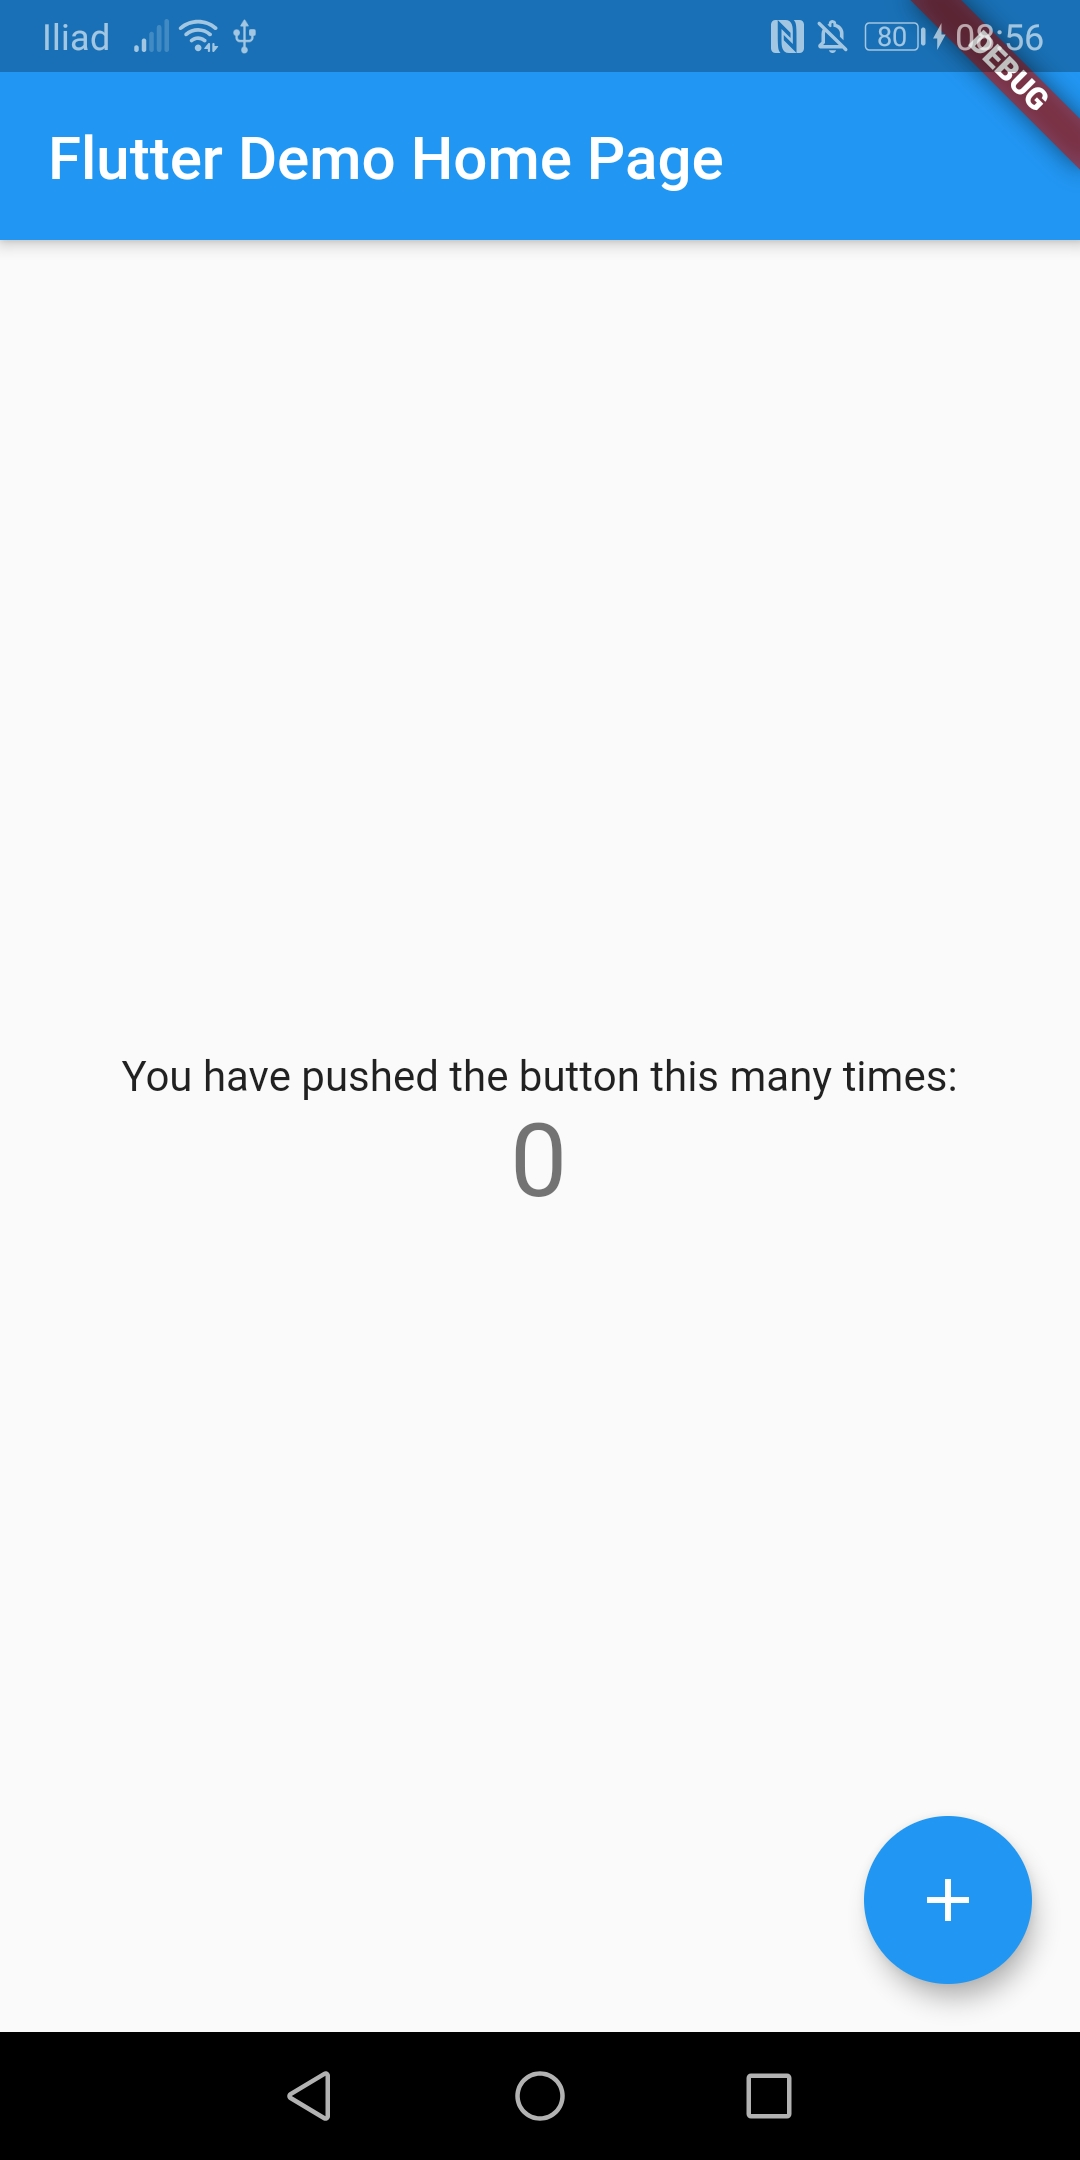
\includegraphics[width=6cm]{immagini/base.jpeg}
	\caption{Applicazione base}
	\label{fig:Applicazione base}
\end{figure}

\newpage

\subsubsection{Applicazione 1}
Questa applicazione permette di rispondere a una serie di domande e successivamente, a quiz terminato, ci sarà una valutazione finale in base alle risposte assegnate.\\
Una volta terminato, il quiz può essere ritentato.\\
In particolare la creazione di questa applicazione mi ha permesso di apprendere meglio il funzionamento di alcuni widget fondamentali.\\
Tra questi sono stati visti principalmente i seguenti: AppBar, Text, Container, ElevatedButton.\\
Inoltre mi ha permesso di capire gli attributi dei widget precedentemente elencati e mi ha fatto comprendere il funzionamento dello \textit{setState()}.\\

\begin{figure}[htbp]	
	\centering
	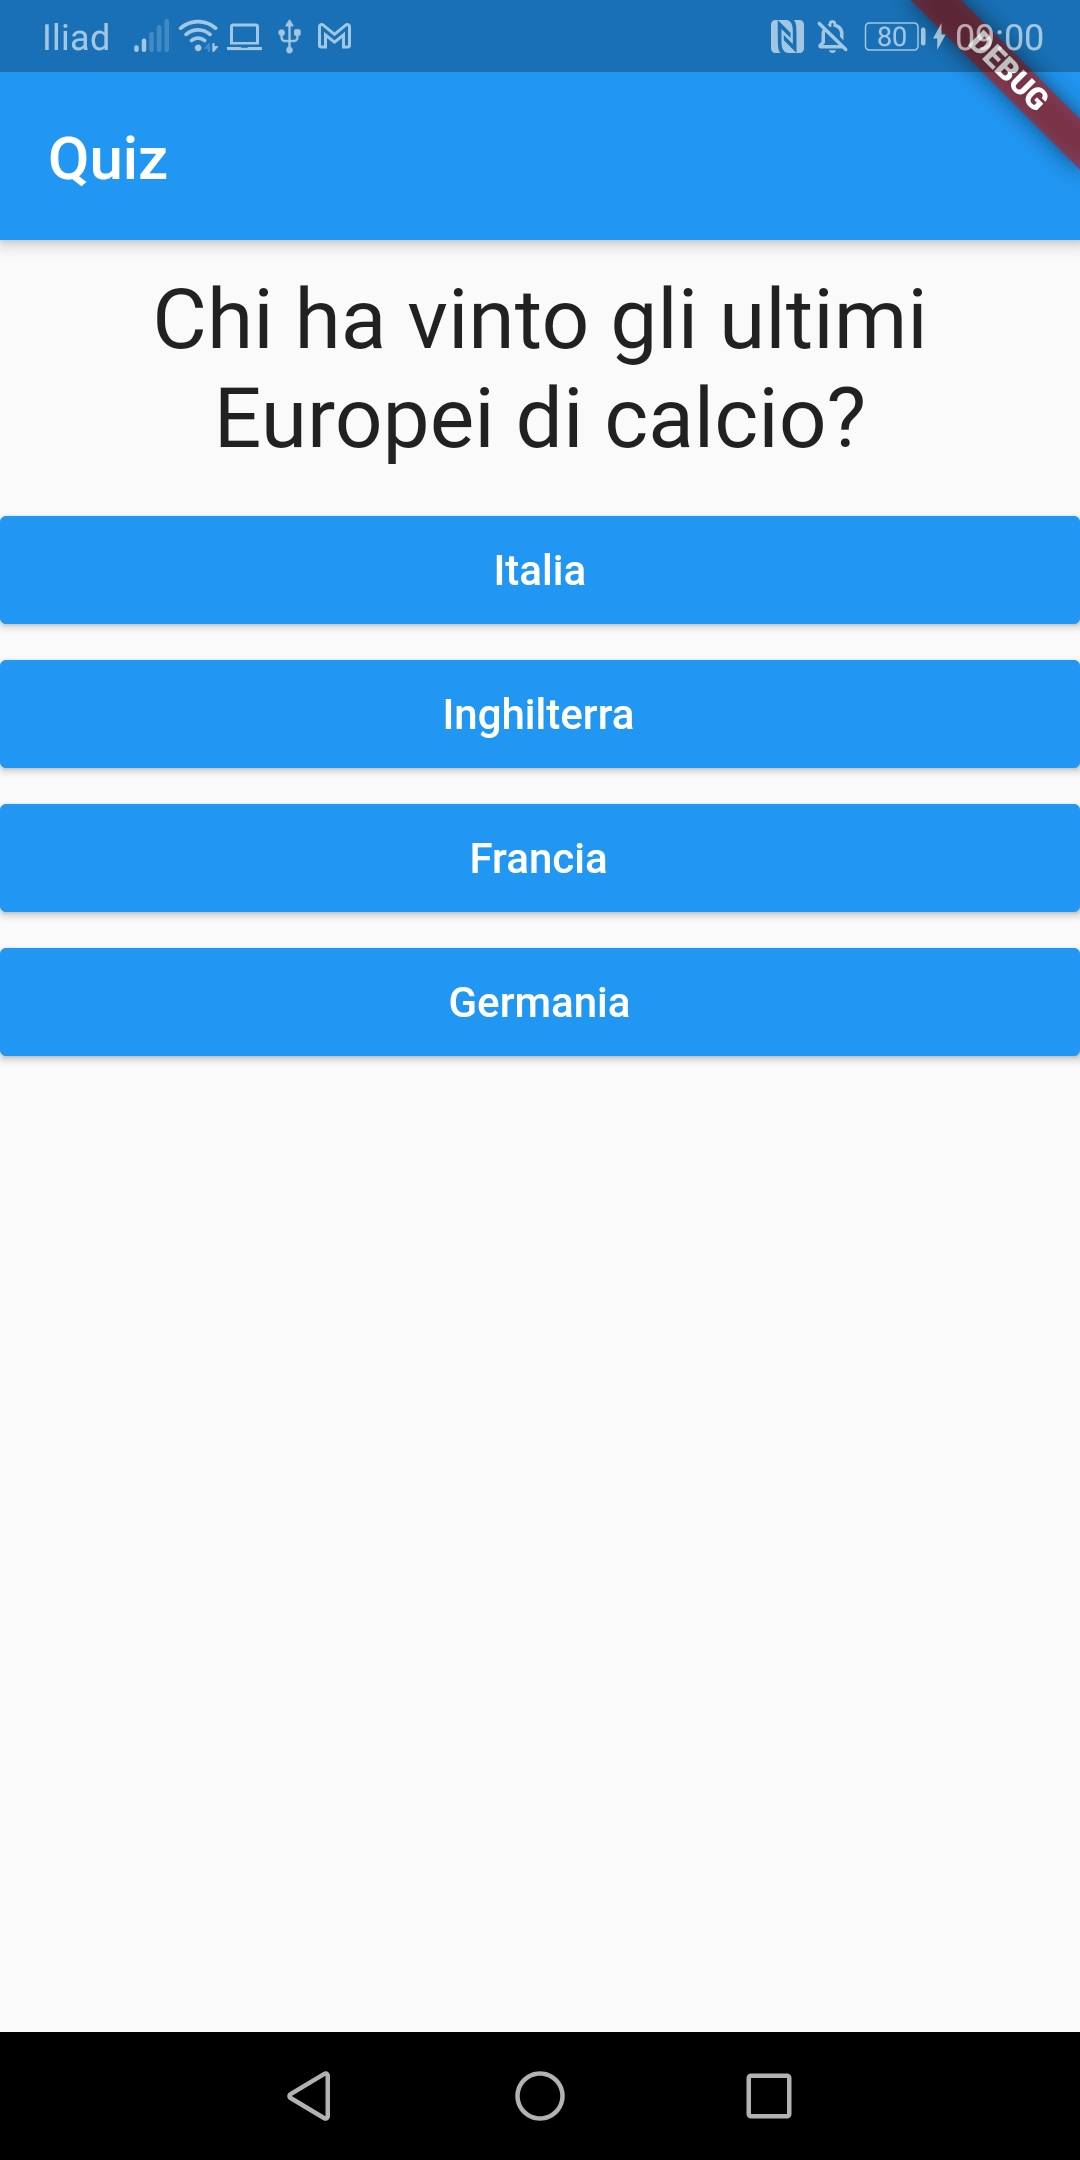
\includegraphics[width=6cm]{immagini/app1.jpeg}
	\caption{Applicazione 1}
	\label{fig:Applicazione 1}
\end{figure}

\newpage

\subsubsection{Applicazione 2}
Questa applicazione permette di inserire delle transizioni che un utente ha effettuato così da monitorare le spese sostenute.\\
In particolare mi ha permesso di comprendere alcuni attributi e widget più complessi rispetto a quelli base, studiare per bene il layout in modo che si adattasse alle dimensioni del cellulare, configurare una pagina in modo scrollabile e gestire widget a comparsa.\\

\begin{figure}[htbp]	
	\centering
	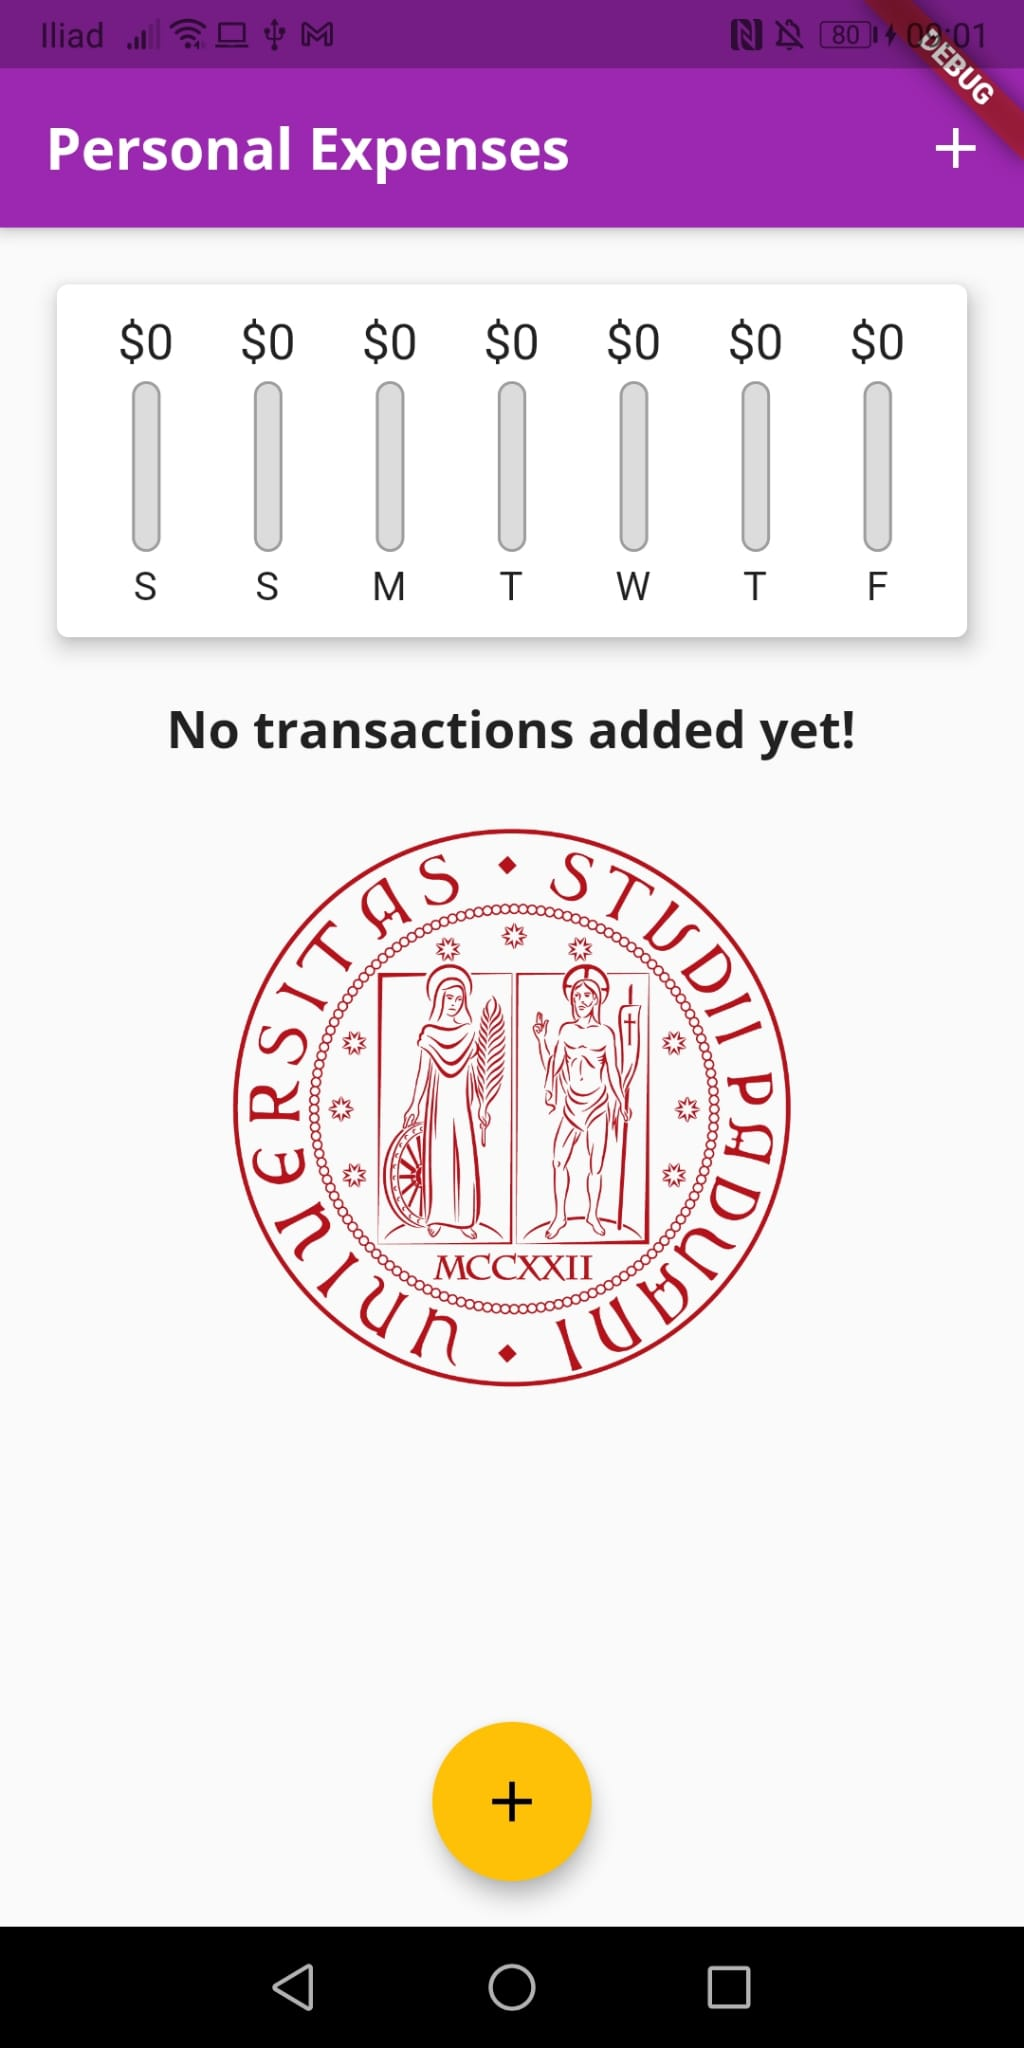
\includegraphics[width=6cm]{immagini/app2.jpeg}
	\caption{Applicazione 2}
	\label{fig:Applicazione 2}
\end{figure}

\newpage

\subsubsection{Applicazione 3}
Quest'ultima applicazione permette di gestire diverse categorie di cibo, i quali contengono diverse ricette che possono essere aggiunte ai preferiti.\\
In particolare mi ha permesso di capire il corretto funzionamento delle Card, delle liste e come gestire nel menu laterale(drawer) i preferiti e i filtri.\\

\begin{figure}[htbp]	
	\centering
	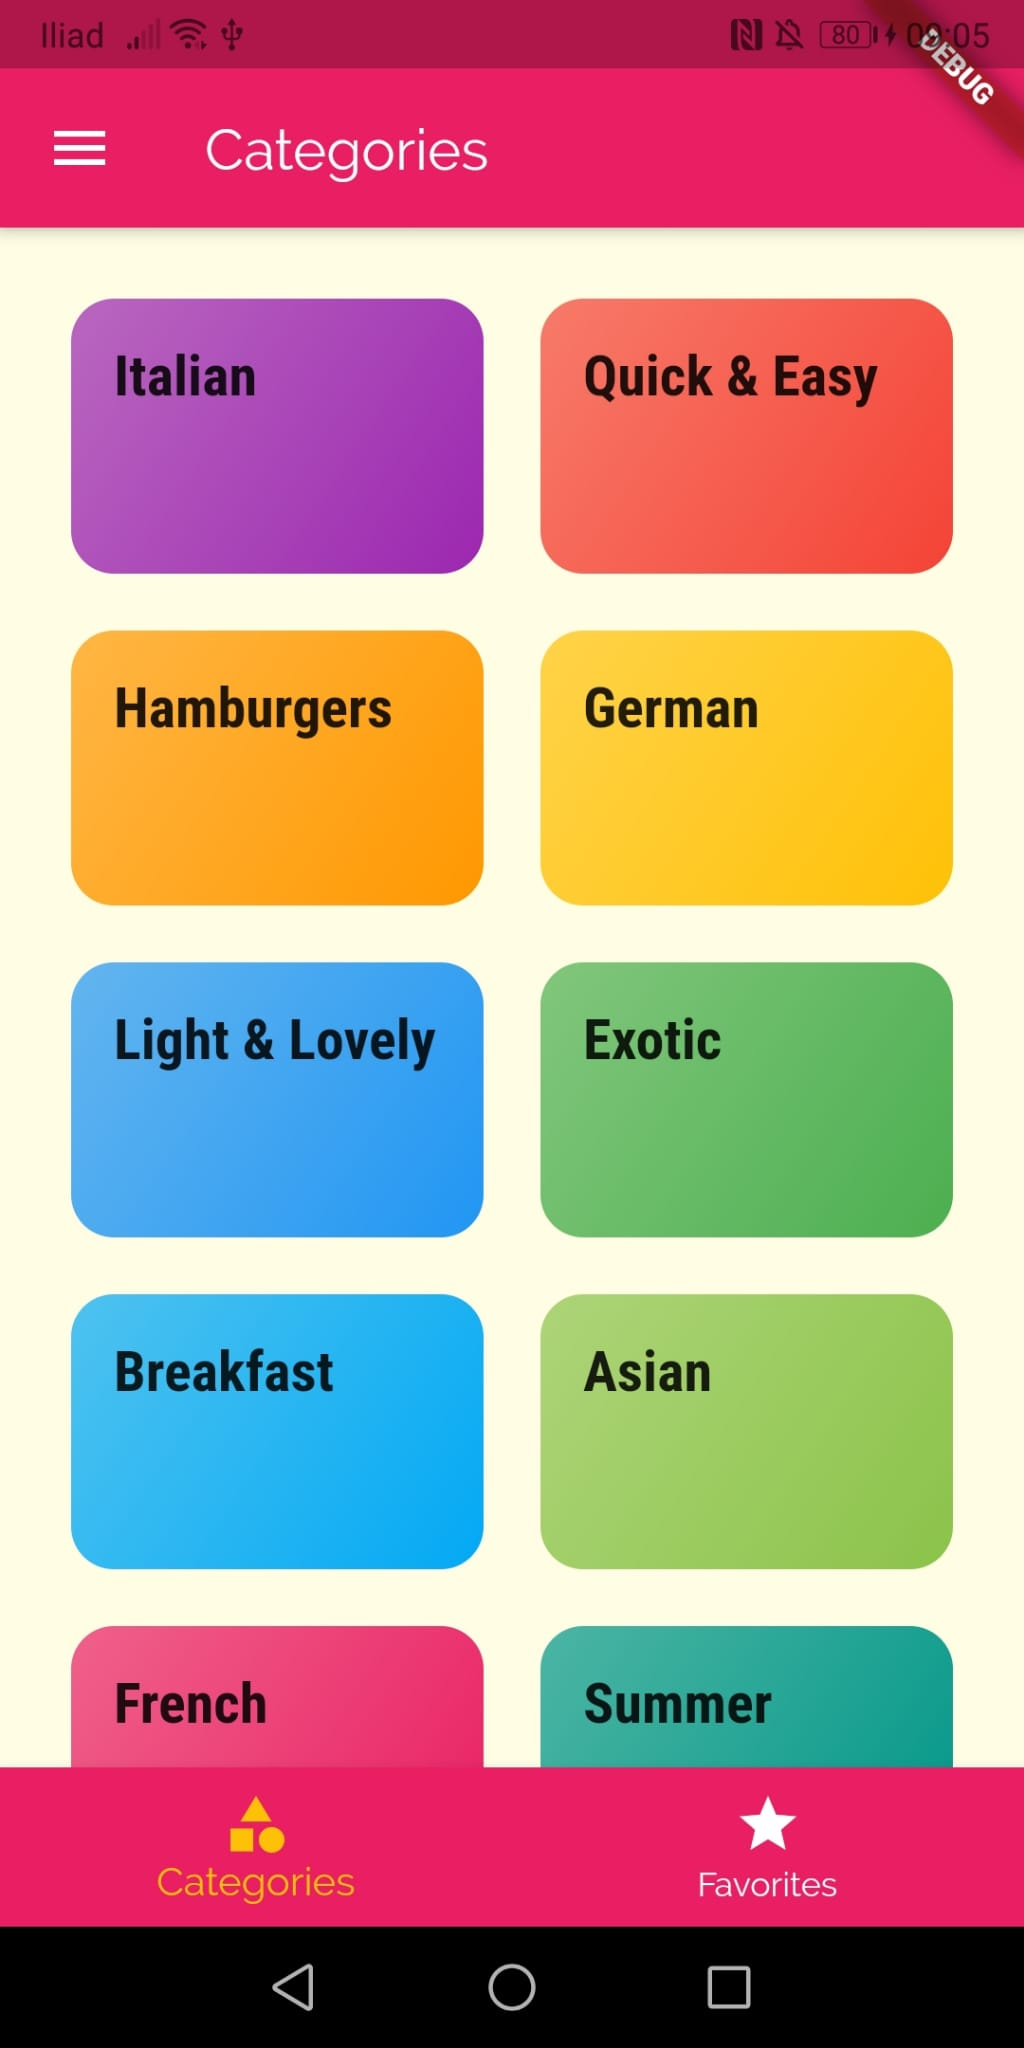
\includegraphics[width=6cm]{immagini/app3.jpeg}
	\caption{Applicazione 3}
	\label{fig:Applicazione 3}
\end{figure}






             % Kick-Off
% !TEX encoding = UTF-8
% !TEX TS-program = pdflatex
% !TEX root = ../tesi.tex

%**************************************************************
\chapter{Sportwill}
\label{cap:Sportwill}
%**************************************************************

\intro{In questo capitolo viene descritto il progetto, le tecnologie e gli strumenti utilizzati. Viene inoltre effettuata un'analisi dei requisiti per poi definire come le varie funzionalità sono state implementate. }\\

%**************************************************************

\section{Descrizione progetto}
Sportwill è un'applicazione che permette di gestire eventi sportivi.\\
Dopo essersi autenticati al sistema si possono visualizzare tutte le attività presenti, passate e future attraverso delle card.\\
 È possibile cercare queste attività utilizzando vari filtri presenti oppure scorrendo la pagina.\\ 
 Ogni utente può gestire i propri eventi creando nuove attività e modificandole successivamente nell'apposita sezione.\\
 Una volta che un utente vuole far partire un nuovo evento dovrà andare sulle specifiche dell'attività e premere sull'apposito bottone per farla iniziare e successivamente la medesima potrà essere messa anche in pausa.\\
 Una volta iniziata l'attività, verranno presi i dati relativi alla posizione così da poter far vedere agli altri utenti in una mappa la posizione in tempo reale.\\
 Grazie a questa mappa gli altri utenti premendo sull'apposito bottone segnaleranno a chi ha fatto partire l'evento che vogliono partecipare anche loro così da poterlo raggiungere.
 
 \newpage
 
 Di seguito vengono riportate due immagini dell'applicazione.\\
 La prima rappresenta la pagina principale dell'applicazione alla quale si arriva dopo essersi autenticati al sistema mentre la seconda rappresenta i dettagli di una nuova attività alla quale posso partecipare premendo sul bottone \textit{Partecipo anche io!}.\\
 
\begin{figure}[htbp]
	\begin{minipage}[b]{0.47\textwidth}
		\centering
		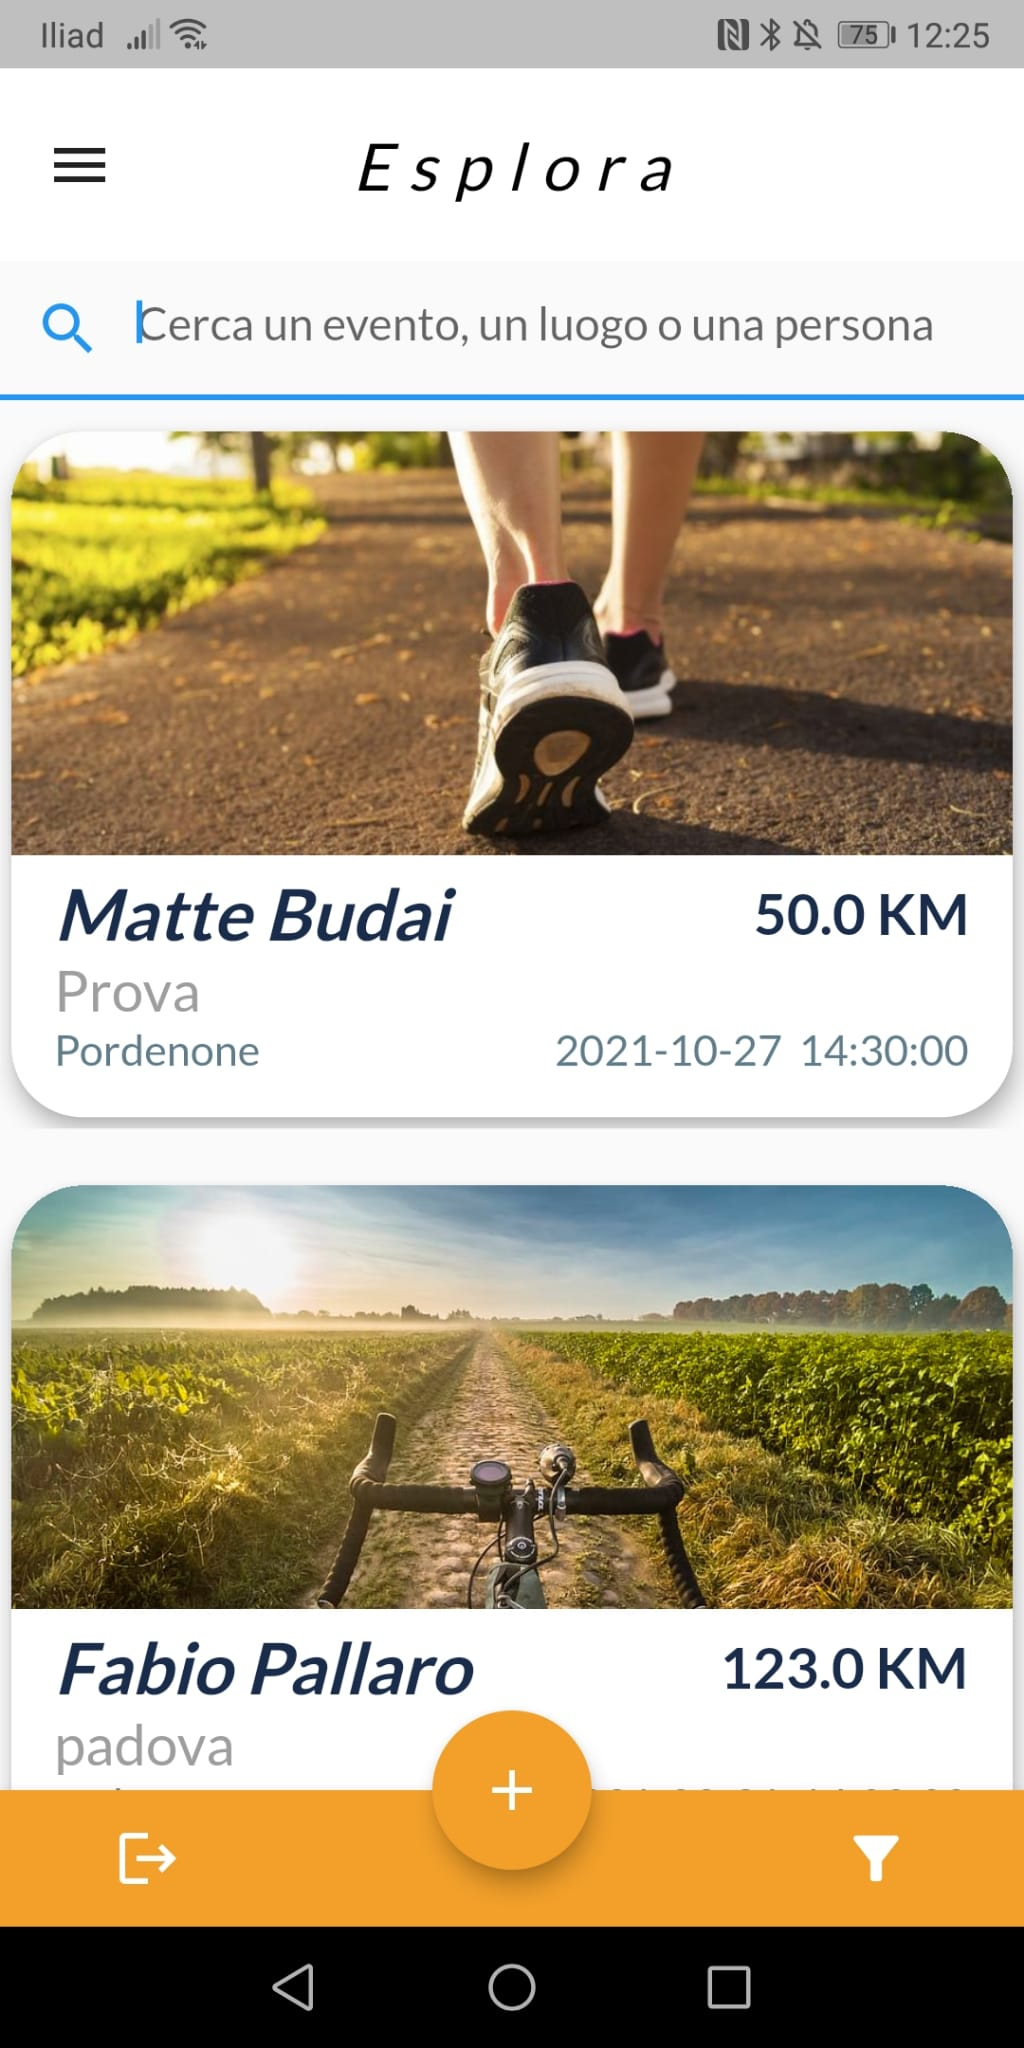
\includegraphics[width=6cm]{immagini/colori.jpeg}
		\caption{Pagina principale}
		\label{fig:Pagina principale}
	\end{minipage}
	\hfill
	\begin{minipage}[b]{0.47\textwidth}
		\centering
		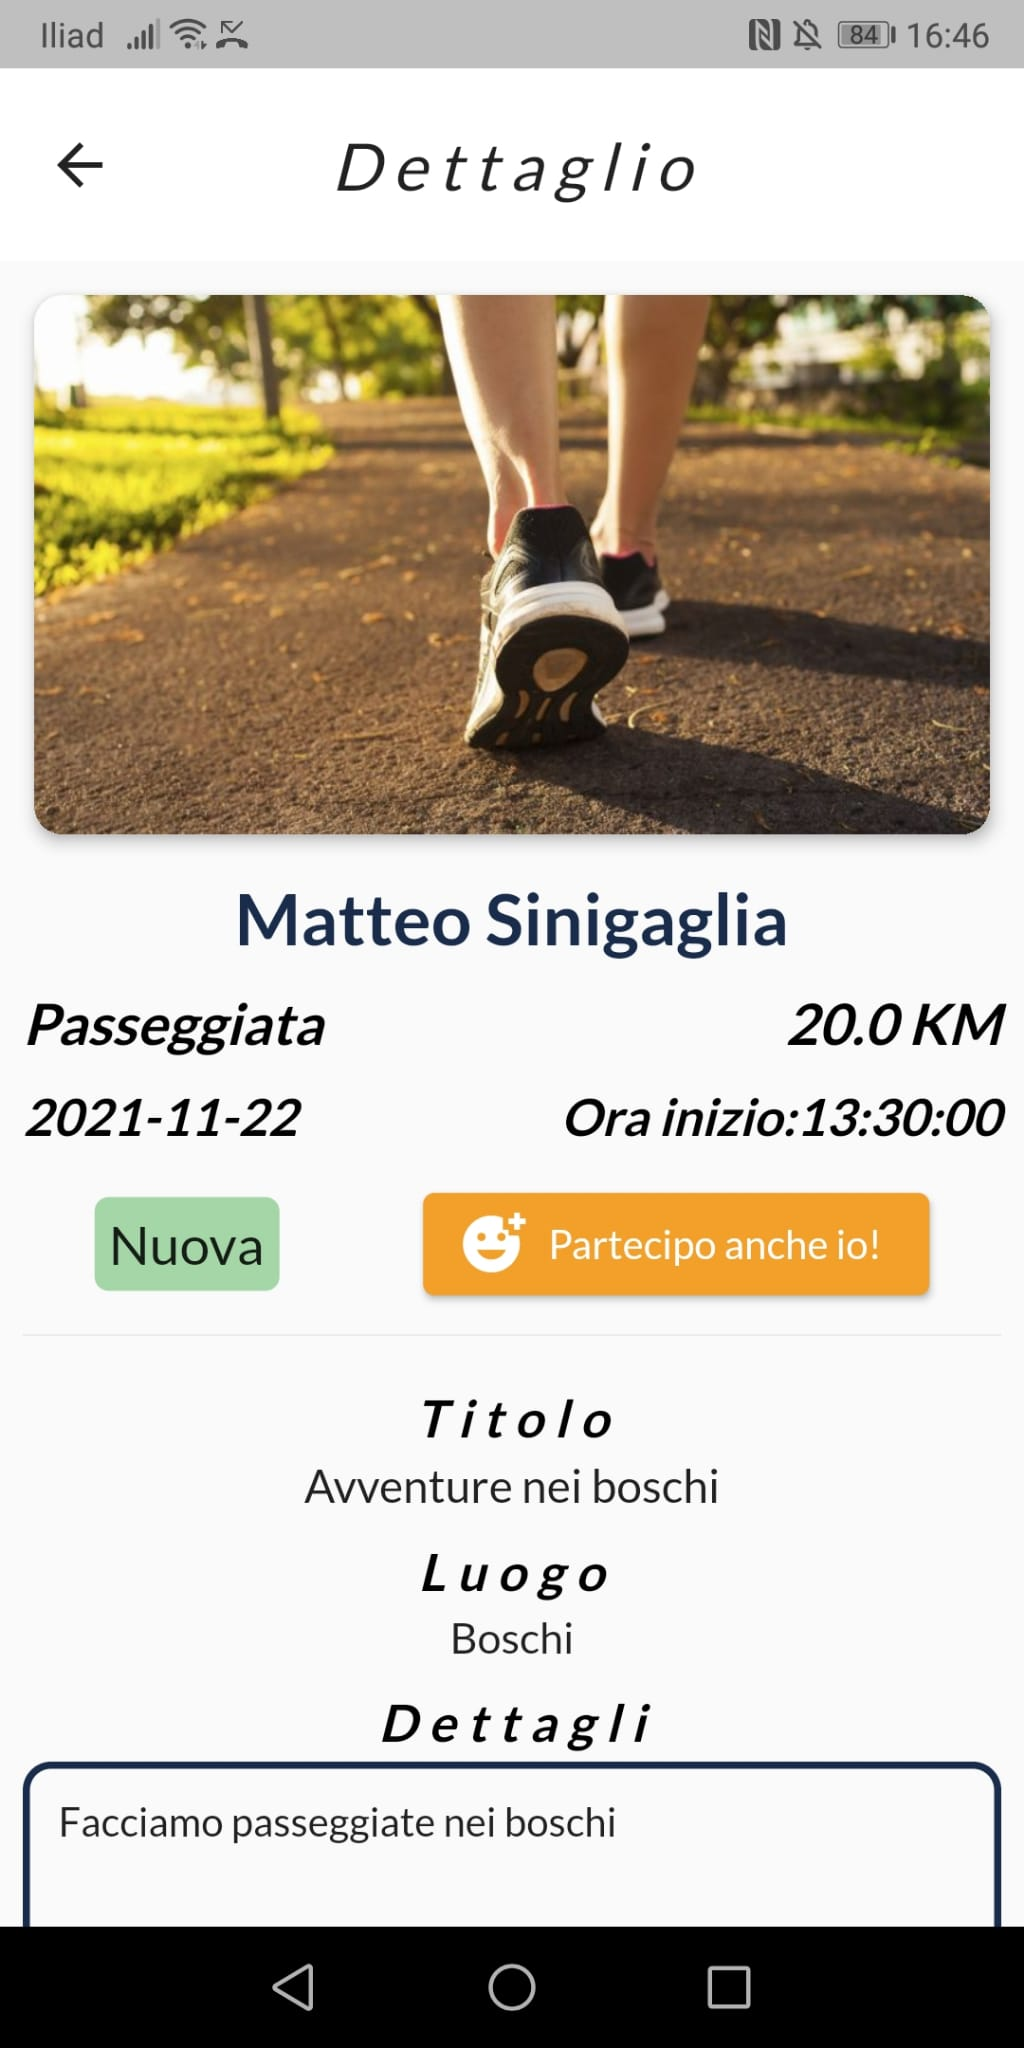
\includegraphics[width=6cm]{immagini/partecipo.jpeg}
		\caption{Schermata di partecipazione}
		\label{fig:Schermata di partecipazione}
	\end{minipage}
\end{figure}
 
 \newpage

\subsection{Organizzazione del progetto}

All'interno del progetto i file sono stati suddivisi nel varie sottocartelle in base al loro compito.\\
Oltre al file main.dart, che è il file principale dell'applicazione, sono presenti altre 4 cartelle che permettono di organizzare meglio il lavoro:
\begin{itemize}
	\item \textbf{models}: che permette di gestire le eccezioni;
	\item \textbf{providers}: che permette di gestire il modello dei dati e fare le varie chiamate al backend;
	\item \textbf{screens}: che crea tutte le pagine dell'applicazione con gli appositi widget;
	\item \textbf{widgets}: che offrono supporto agli screens tramite la creazione di widget.
\end{itemize}
\begin{figure}[htbp]	
	\centering
	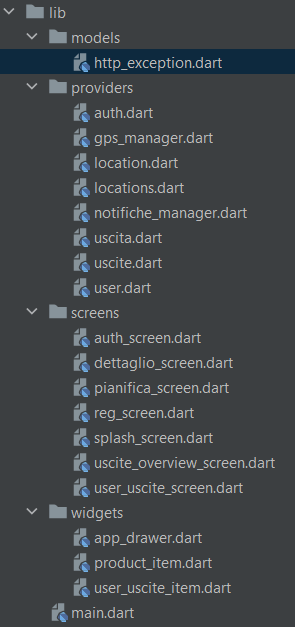
\includegraphics[width=5cm]{immagini/struttura.png}
	\caption{Struttura progetto}
	\label{fig:Struttura progetto}
\end{figure}

\newpage

\section{Tecnologie e strumenti}
Per svolgere il progetto, tralasciando lo studio del framework Flutter e del linguaggio Dart che vengono descritti nel capitolo precedente, è stato necessario utilizzare altri strumenti e tecnologie.\\
Tra questi i principali sono:
\begin{itemize}
	\item Android Studio;
	\item GitLab;
	\item Database DBeaver;
	\item Backend Spring.
\end{itemize}

\subsection{Android Studio}
Android Studio è un IDE per lo sviluppo per la piattaforma Android.\\
Questo IDE, già utilizzato da me in precedenza, è stato configurato correttamente installando i plugin per Flutter e Dart necessari.\\
Android Studio mi ha permesso inoltre di installare e configurare il cellulare così da poter vedere l'applicazione in modo realistico sul mio dispositivo fisico.\\
È molto valido anche perchè fornisce vari dispositivi virtuali su cui testare l'applicazione.

\begin{figure}[htbp]	
	\centering
	
\includegraphics[width=3cm]{immagini/logoandroidstudio.png}
	\caption{Logo Android Studio}
	\label{fig:Logo Android Studio}
\end{figure}

\subsection{GitLab}
GitLab è una piattaforma web open source che permette la gestione di repository Git.\\
Grazie a GitLab è possibile lavorare parallelamente
ad altre persone sullo stesso progetto senza generare conflitti.\\
All'interno della repository presente su GitLab al seguente indirizzo \url{https://gitlab.synclab.it/padovaformazione/sportwill/} viene gestito tutto il progetto ovvero il backend, l'applicazione mobile e la webapp.\\

\begin{figure}[htbp]	
	\centering
	
\includegraphics[width=2cm]{immagini/logogitlab.png}
	\caption{Logo GitLab}
	\label{fig:Logo GitLab}\end{figure}

\newpage

\subsection{Database}
Il database utilizzato per l'applicazione è DBeaver che è gratuito e scaricabile alla seguente pagina \url{https://dbeaver.io/download/}.\\
L'utilizzo del database è stato fondamentale per testare che tutto andasse nella maniera prevista.\\

\begin{figure}[htbp]	
	\centering
	
\includegraphics[width=3cm]{immagini/logodbeaver.png}
	\caption{Logo DBeaver}
	\label{fig:Logo DBeaver}
\end{figure}

\subsection{Backend}
Per gestire i dati sono state fatte delle chiamate al backend.\\
Il backend comprendeva principalmente i linguaggi Spring boot e Spring jpa ed è stato gestito da altri stagisti con il quale sono stato in stretto contatto per organizzare le varie chiamate necessarie, così da definire gli indirizzi e i valori attesi.\\
Tutto queste chiamate erano disponibili su un server gestito dal tutor aziendale Fabio Pallaro.\\

\begin{figure}[htbp]	
	\centering
	
\includegraphics[width=3cm]{immagini/springlogo.png}
	\caption{Logo Spring}
	\label{fig:Logo Spring}
\end{figure}

\newpage

\section{Analisi dei requisiti}
In questa sezione viene descritta l'analisi dei requisti con i  vari casi d'uso individuati e successivamente viene effettuato il tracciamento.

\subsection{Casi d'uso}
In un primo momento per determinare i casi d'uso sono stati definiti gli attori principali dell'applicazione.
Tra questi sono state identificate tre tipologie:
\begin{itemize}
	\item Utente non autenticato;
	\item Utente autenticato;
	\item Utente ospite.
\end{itemize}
Successivamente sono stati definiti i quattro casi d'uso:
\begin{itemize}
	\item Visualizzazione mappa;
	\item Visualizzazione mappa schermo intero;
	\item Filtro base;
	\item Filtro avanzato.
\end{itemize}


\subsubsection{ UC1 - Visualizzazione mappa}

	\textbf{Attori Primari:} Utente autenticato e utente ospite.\\
	\textbf{Descrizione:} L'utente vuole vedere la mappa dell'attività selezionata.\\
	\textbf{Scenario principale:} L'utente si trova nella schermata principale dell'applicazione e preme sulla card dell'attività a cui è interessato. Se questa attività è iniziata e contiene dati relativi alla posizione verrà mostrata la mappa altrimenti non comparirà tra i dettagli.\\
	\textbf{Precondizione:} L'utente si trova nella schermata principale dell'applicazione e preme su una card.\\
	\textbf{Postcondizione:} Se l'attività selezionata conterrà dati relativi alla posizione verrà mostrata una mappa con punto di partenza, percorso svolto e punto attuale o finale.\\


\subsubsection{ UC2 - Visualizzazione mappa schermo intero}

\textbf{Attori Primari:} Utente autenticato e utente ospite.\\
\textbf{Descrizione:} L'utente vuole vedere la mappa a schermo intero per navigare meglio.\\
\textbf{Scenario principale:} L'utente sta visualizzando le specifiche di un'attività e tra queste è presente pure la mappa, per poter usare in modo più confortevole la mappa deve poter premere su un bottone che la ingrandisce a schermo intero.\\
\textbf{Precondizione:} L'utente si trova nelle specifiche di un'attività e tra i dettagli e presente anche la mappa. Una volta individuata preme sul bottone per renderla a schermo intero.\\
\textbf{Postcondizione:} La mappa viene visualizzata a schermo intero così da facilitarne l'utilizzo.\\

\subsubsection{ UC3 - Filtro base}

\textbf{Attori Primari:} Utente autenticato e utente ospite.\\
\textbf{Descrizione:} L'utente cerca un'attività in base al luogo, al titolo e alla persona che l ha creata digitando su una casella di ricerca.\\
\textbf{Scenario principale:} L'utente si trova nella pagina principale dell'applicazione e vuole cercare l'attività effettuata da un altro utente. Per cercarla basterà che inizierà a digitare il nome o il cognome della persona desiderata e compariranno solo le card che contengono quanto appena scritto.\\
\textbf{Precondizione:} L'utente si trova nella pagina principale dell'applicazione e inizia a scrivere nella casella di ricerca.\\
\textbf{Postcondizione:} Vengono visualizzate solo le card che contengono nel titolo, nel nome, nel cognome o nel titolo quello scritto dall'utente.\\

\subsubsection{ UC4 - Filtro avanzato}

\textbf{Attori Primari:} Utente autenticato e utente ospite.\\
\textbf{Descrizione:} L'utente si trova nella pagina principale dell'applicazione e aprendo il menù dei filtri può applicarli in base alle sue esigenze.\\
\textbf{Scenario principale:} L'utente apre il menù dei filtri e seleziona la data di inizio o lo sport che gli interessano e preme sull'icona del check per applicarli così da vedere solo le card con quella tipologia di sport e apartire da quella data.\\
\textbf{Precondizione:} L'utente si trova nel menù dei filtri, riempa alcuni campi e preme sull'icona del check.\\
\textbf{Postcondizione:} L'utente visualizza solo le card che rispettano i valori messi nel filtro in precedenza. Per aiutare l'utente e far capire che il filtro è stato applicato, l'icona che porta al menù dei filtri cambia colore in verde.\\

\newpage

\subsection{Tracciamento requisti}
I requisiti individuati sono tutti fondamentali e obbligatori e possono essere:
\begin{itemize}
	\item \textbf{Funzionali}: legati alle funzionalità offerte dal sistema;
	\item \textbf{Qualitativi}: rappresentanti standard e metriche da seguire per garantire la qualità del sistema;
	\item \textbf{Di Vincolo}: dipendenti da fattori esterni o di dominio.
\end{itemize}
Per ogni requisito delle tabelle sottostanti è stata decisa la seguente struttura: 
\begin{itemize}
	\item\textbf{Requisito:} R[Tipologia][Identificativo];
	\item\textbf{Descrizione:} descrizione breve ma completa del requisito, meno ambigua possibile;
	\item\textbf{Fonti:} ogni requisito può derivare dalle seguenti fonti:
	\begin{itemize}
		\item Azienda: si tratta di un requisito individuato con l'azienda;
		\item Caso d'uso: si tratta di un requisito estrapolato dai casi d'uso individuati.
	\end{itemize}
\end{itemize}

\subsubsection{Requisiti funzionali}

\begin{center}
	\begin{table}[h!]
		
		\label{tab:Requisiti funzionali}
		\begin{tabularx}{\textwidth}{|c|p{8cm}|p{2.1cm}|}
			
			\hline
			\textbf{Requisito} & \centering\textbf{Descrizione} & \textbf{Fonti}  \\\hline
			
			R1F1 & Se ci sono coordinate relative alla posizione per un'attività deve essere possibile visualizzare la mappa  & UC1\\
			\hline	
			R1F2 &Deve essere possibile visualizzare la mappa a schermo intero. & UC2\\
			\hline
			R1F3& Deve essere possibile cercare le attività per titolo, luogo, nome e cognome.	& UC3	\\
			\hline	
			R1F4& Deve essere possibile applicare filtri avanzati all'attività che comprendono il tipo di sport, la data di inizio, di fine e se si riferiscono ad attività che ho creato io.	& UC4	\\
			\hline		
		\end{tabularx}
		\vspace{0.3cm}
		\caption{Requisiti funzionali}
	\end{table}
\end{center}

\newpage

\subsubsection{Requisiti qualitativi}

\begin{center}
	\begin{table}[h!]
		
		\label{tab:Requisiti qualitativi}
		\begin{tabularx}{\textwidth}{|c|p{8cm}|p{2.1cm}|}
			
			\hline
			\textbf{Requisito} & \centering\textbf{Descrizione} & \textbf{Fonti}  \\\hline
			
			R1Q1 &Il codice scritto dovrà essere versionabile tramite Git.  & Azienda\\
			\hline	
			R1Q2 &Il repository utilizzato sarà quello presente su GitLab. & Azienda\\
			\hline
			R1Q3& Per implementare le funzionalità bisognerà usare il framework Flutter con linguaggio Dart.	& Azienda	\\
			\hline		
		\end{tabularx}
		\vspace{0.3cm}
		\caption{Requisiti qualitativi}
	\end{table}
\end{center}

\subsubsection{Requisiti di vincolo}

\begin{center}
	\begin{table}[h!]
		
		\label{tab:Requisiti di vincolo}
		\begin{tabularx}{\textwidth}{|c|p{8cm}|p{2.1cm}|}
			
			\hline
			\textbf{Requisito} & \centering\textbf{Descrizione} & \textbf{Fonti}  \\\hline
			
				R1V1 & Tutti i dati dovranno essere memorizzati nel back-end.  & Azienda\\
				\hline
				R1V2 & Per le chiamate verrà utilizzato un server fornito dall'azienda.  & Azienda\\
			\hline		
		\end{tabularx}
		\vspace{0.3cm}
		\caption{Requisiti di vincolo}
	\end{table}
\end{center}


\newpage

\section{Implementazioni}
Oltre al completamento dei requisiti sono state effettuate altre implementazioni.\\
Nel complesso le funzionalità realizzate durante lo stage sono state: 
\begin{itemize}
	\item Logo;
	\item Filtro di ricerca testo;
	\item Pagina Modifica e campi obbligatori;
	\item Mappa percorso;
	\item Aggiornamento automatico mappa;
	\item Mappa schermo intero;
	\item Colori;
	\item Pagina Modifica;
	\item Eliminazione, Modifica e Aggiunta di un'attività;
	\item Filtro avanzato di ricerca attività.
\end{itemize}
Tutti i servizi sono stati rilasciati su un'apposita repository aziendale su \textit{GitLab}.

\subsection{Logo}
È stato modificato il logo di base di Flutter con quello di Sportwill.\\
Per  fare ciò è stato inserita l'immagine del logo all'interno della seguente cartella \textit{app/src/main/res/mipmap/}.\\
In alternativa si poteva definire nel file \textit{pubspec.yaml} il percorso del logo dell'applicazione e poi inserire l'immagine del logo nella cartella appena definita.\\

\begin{figure}[htbp]	
	\centering
	
\includegraphics[width=6cm]{immagini/logosportwill.png}
	\caption{Logo Sportwill}
	\label{fig:Logo Sportwill}
\end{figure}

\newpage

\subsection{Filtro di ricerca testo}
All'interno della pagina principale dell'applicazione ovvero la pagina \textit{uscite\_overview\_screen.dart} è stato aggiunto un widget che permette di ricercare le varie card in base all'evento, al luogo o alla persona.\\
Digitando nella barra di ricerca si potranno ricercare solo le card a cui si è interessati.\\
Per fare ciò è stato inserita una funzione chiamata \textit{ricerca()} che ritorna una TextField come Widget nel file \textit{uscite\_overview\_screen.dart}.\\

\begin{figure}[htbp]	
	\centering
	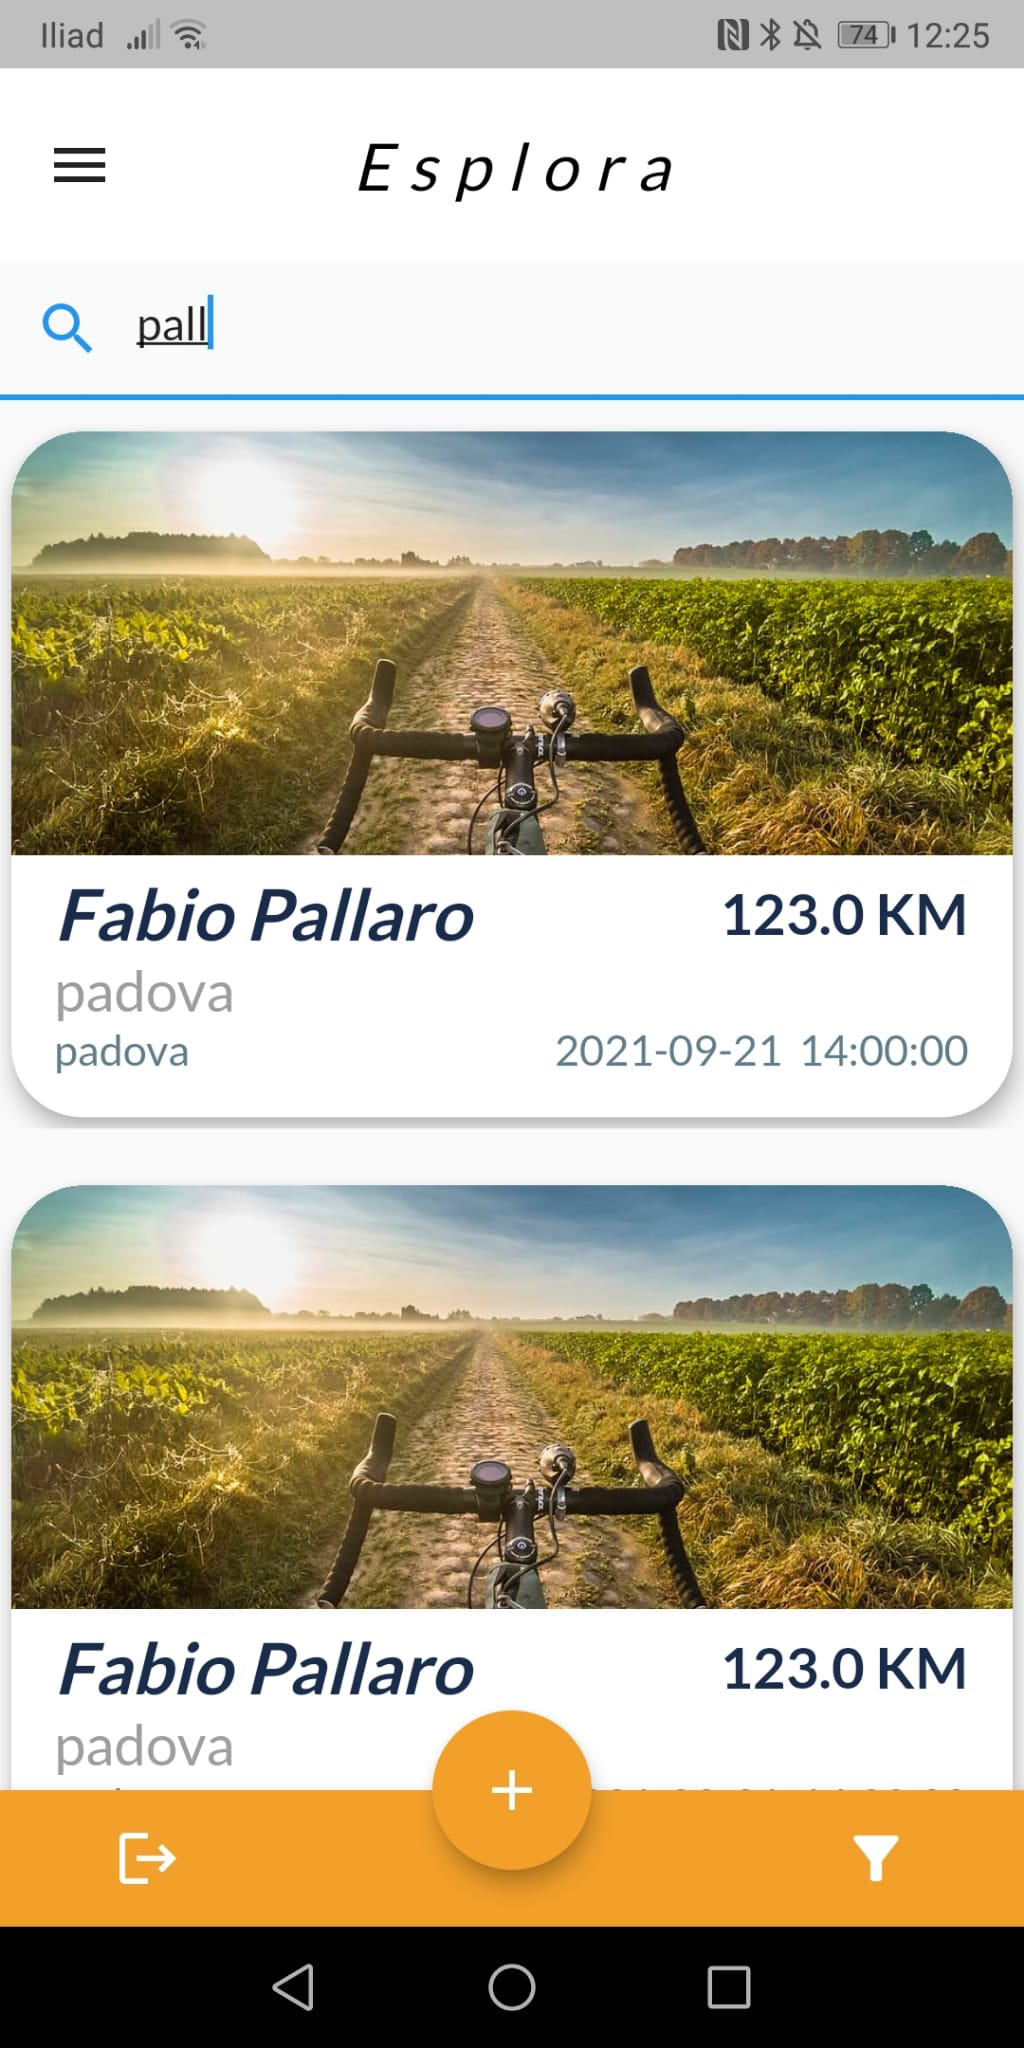
\includegraphics[width=6cm]{immagini/filtrotesto.jpeg}
	\caption{Filtro di ricerca testo}
	\label{fig:Filtro di ricerca testo}
\end{figure}

\newpage

\subsection{Campi obbligatori e pagina modifica e crea}
All'interno di questa pagina sono stati tolti tutti i campi obbligatori non necessari.\\
Per fare ciò sono stati tolti tutti i validator non necessari nel file \textit{pianifica\_screen.dart} e lasciato gli altri validator con le apposite funzioni.\\
Inoltre all'interno di questa pagina sono stati aggiustati i campi degli orari che nella funzione \textit{selezionaOra()} tornava sempre i minuti attuali.\\
Per rendere all'utente più comprensibile il salvataggio è stato sostituita l'icona di salvataggio con l'icona \textit{Icon(Icons.save)}.\\

\begin{figure}[htbp]	
	\centering
	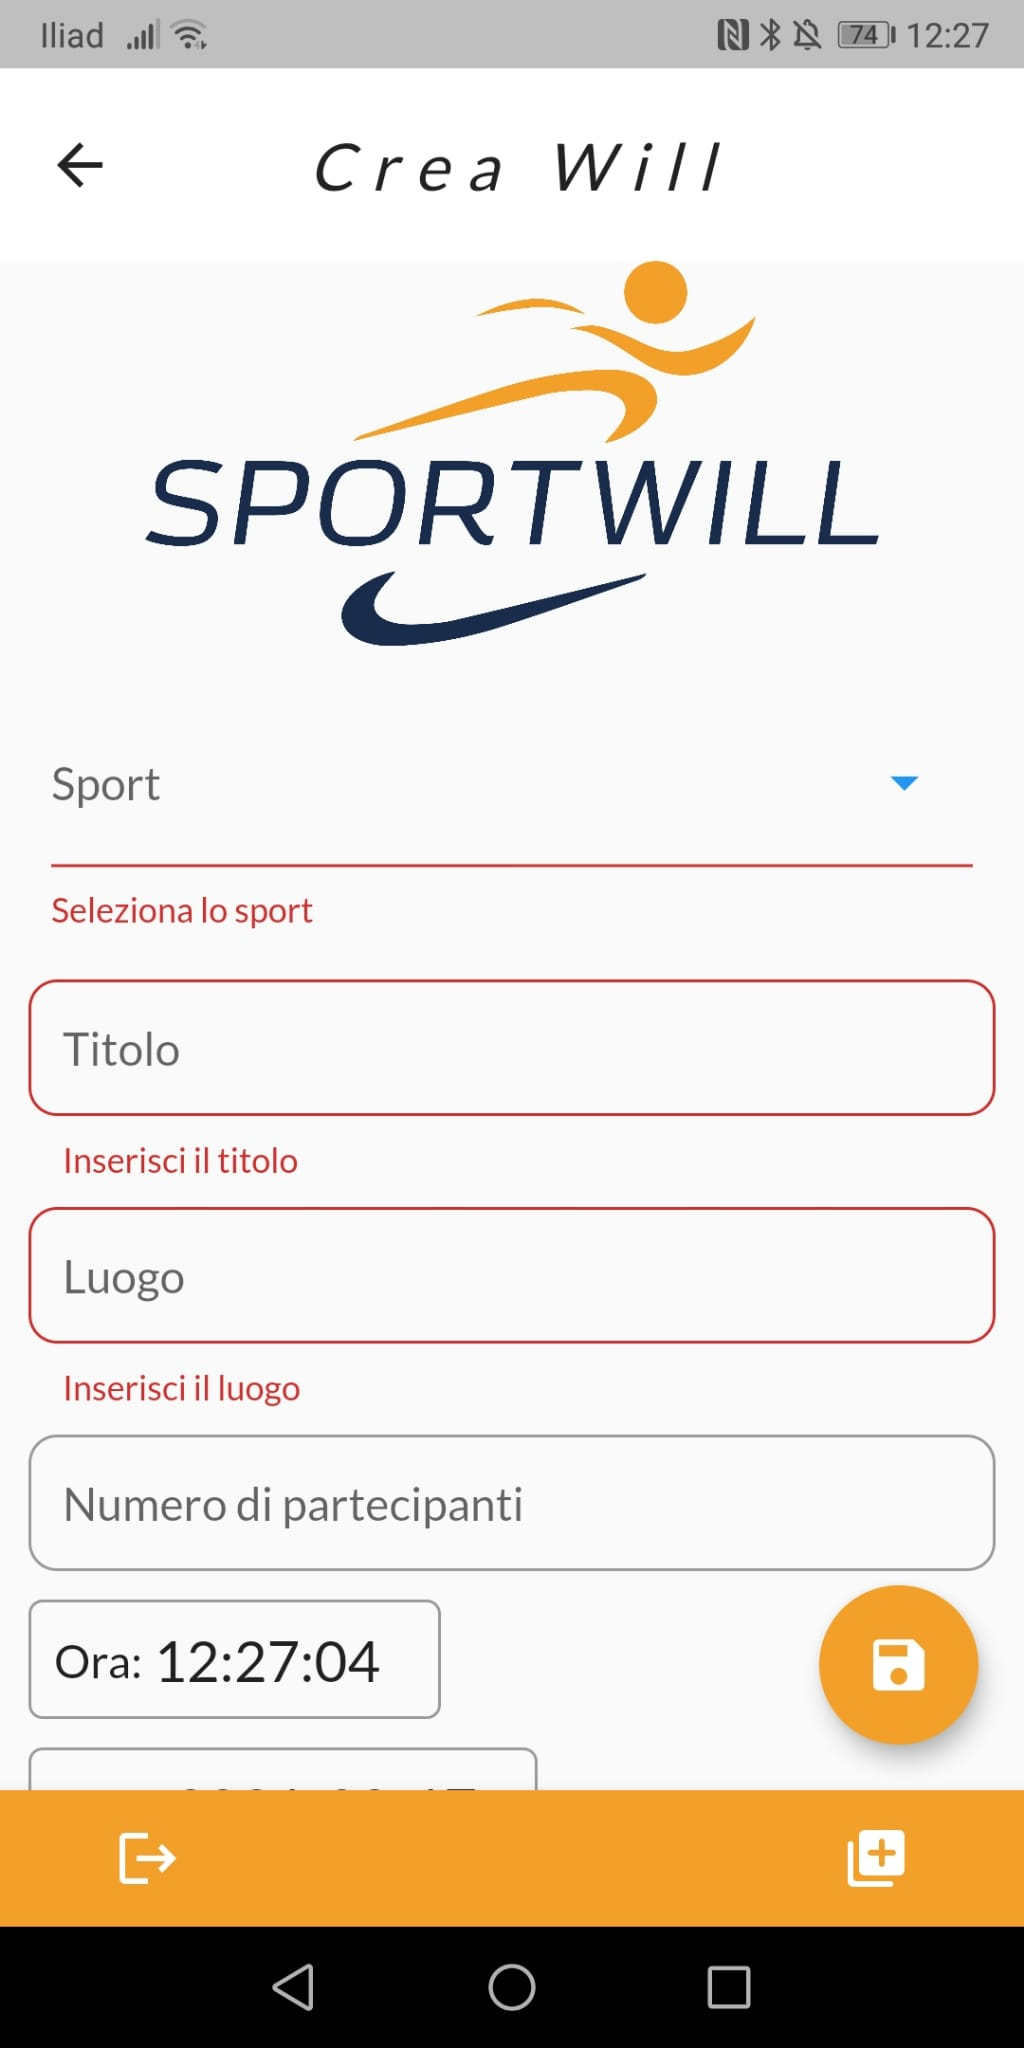
\includegraphics[width=6cm]{immagini/modifica.jpeg}
	\caption{Campi obbligatori}
	\label{fig:Campi obbligatori}
\end{figure}

\newpage

\subsection{Colori}
All'interno dei vari file sono stati cambiati diversi colori in modo che venissero utilizzati principalmente quelli dell'applicazione, ovvero il bianco e l'arancione.\\

\begin{figure}[htbp]	
	\centering
	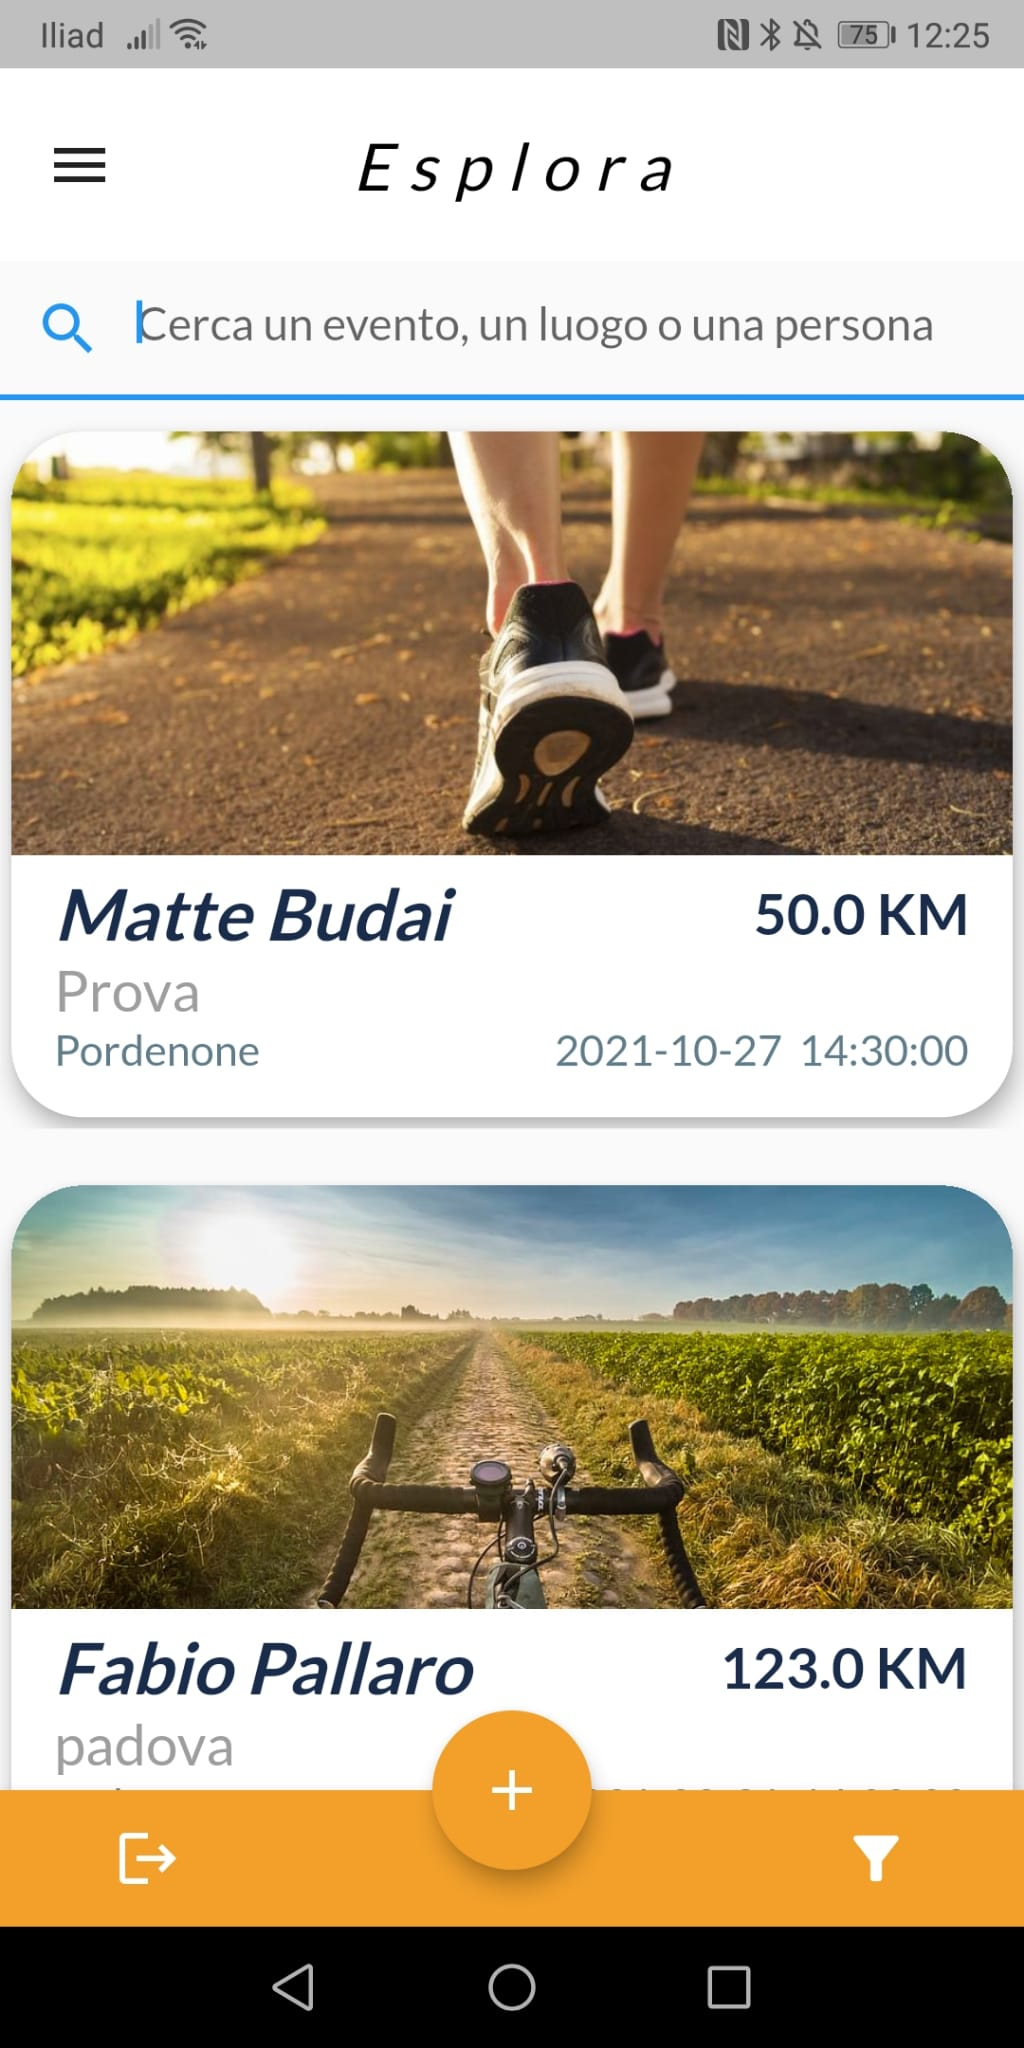
\includegraphics[width=6cm]{immagini/colori.jpeg}
	\caption{Colori}
	\label{fig:Colori}
\end{figure}


\subsection{Eliminazione, Modifica e Aggiunta di un'attività}
In seguito alle modifiche di vari campi sono state sistemate le pagine di eliminazione, modifica e aggiunta di un'attività con nuovi valori e formati in modo che venissero rispettate le richieste del backend.\\
In particolar modo sono stati sistemati i valori che riguardavano la data e l'orario con i nuovi formati richiesti e la lunghezza e il numero di partecipanti che richiedevano un double e un intero.

\newpage

\subsection{Mappa percorso}
Per gestire la mappa sono stati creati due providers:
\begin{itemize}
	\item location.dart: che è il modello e contiene tutti i dati che riguardano una posizione;
	\item locations.dart: che permette di chiamare il backend per ottenere i vari valori da visualizzare nella mappa.
\end{itemize}
La mappa viene creata nel file \textit{dettaglio\_screen.dart} e viene mostrata solo se c'è almeno una posizione per l'attività selezionata.\\
Per visualizzare la mappa viene usato Leaflet e viene creato un array con tutte le posizioni. Queste posizioni vengono poi disegnate sulla mappa mettendo i marker alla prima posizione e all'ultima in ordine temporale.\\

\begin{figure}[htbp]	
	\centering
	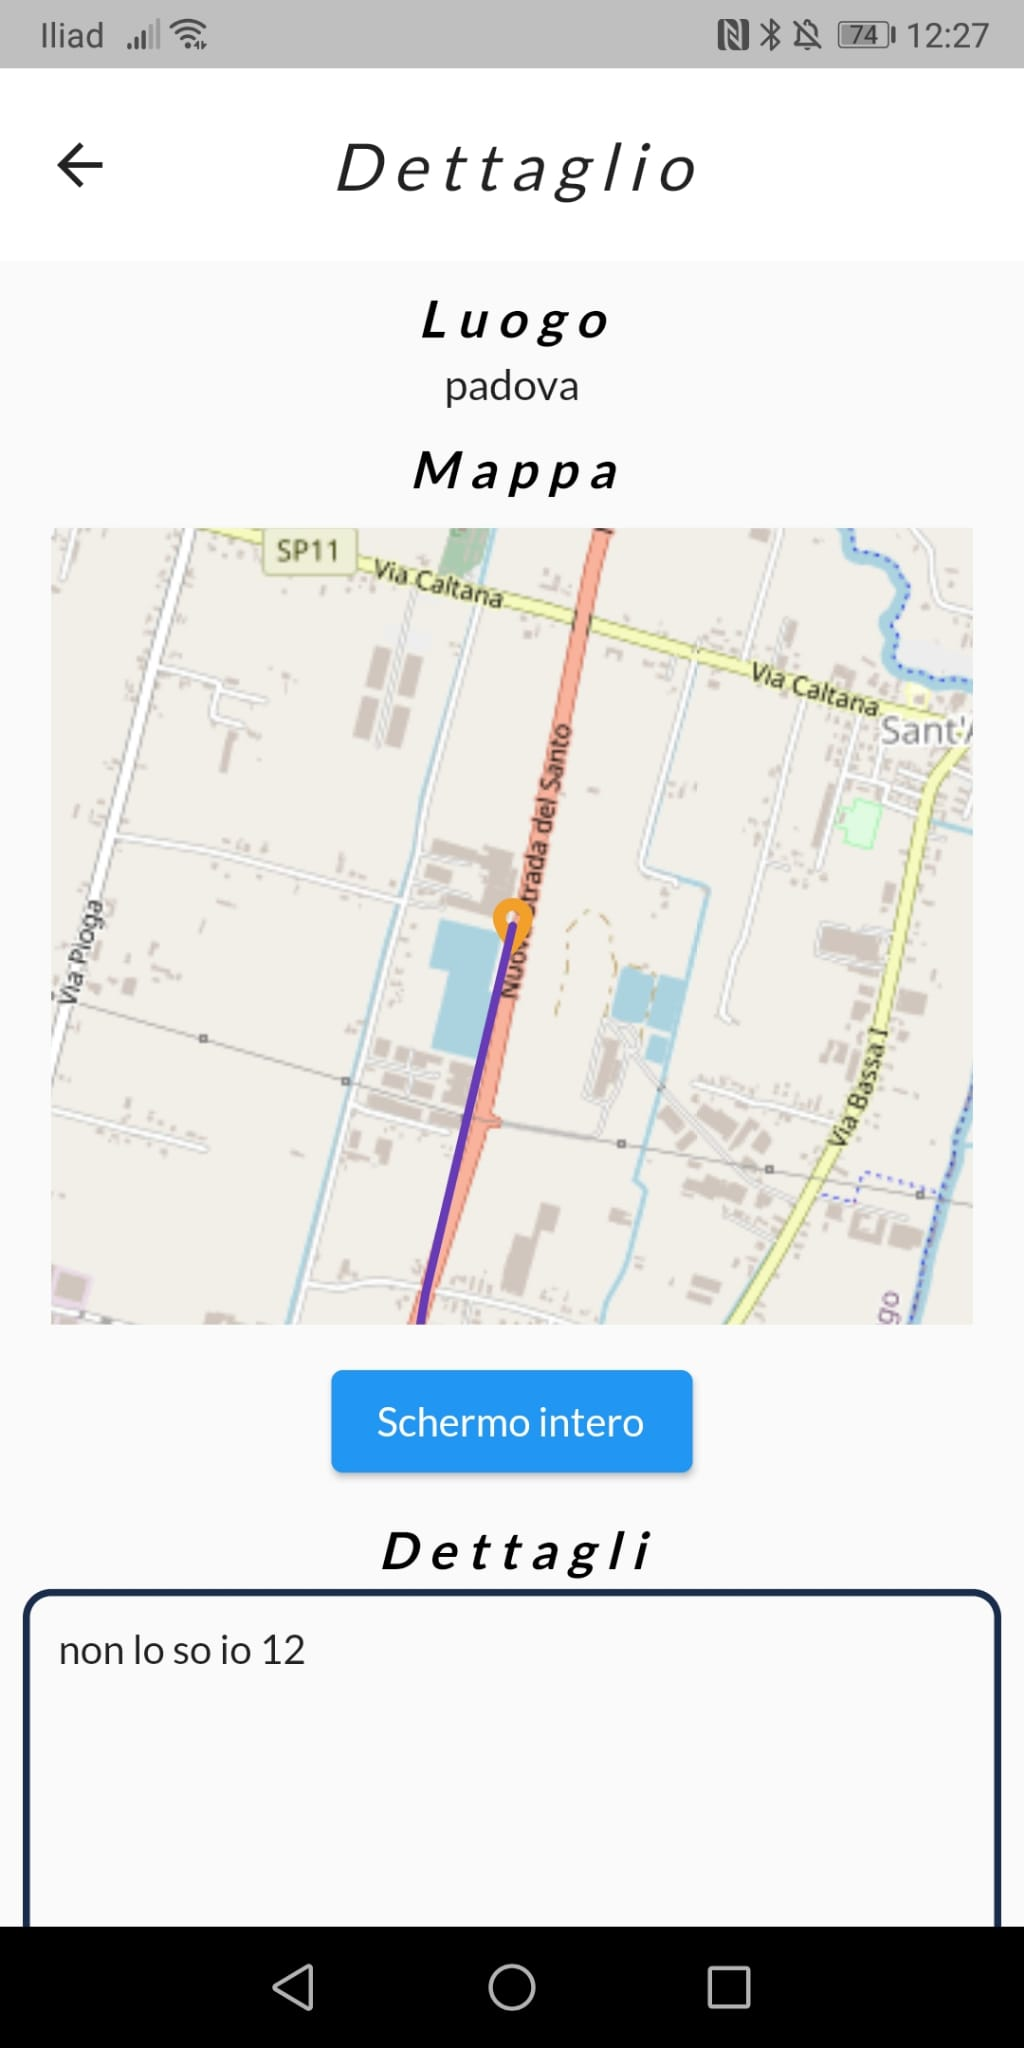
\includegraphics[width=6cm]{immagini/mappa.jpeg}
	\caption{Mappa percorso}
	\label{fig:Mappa percorso}
\end{figure}

\newpage

\subsection{Aggiornamento automatico mappa}
Per fare in modo che la mappa si aggiornasse in modo automatico è stato inserito un Timer che ogni 30 secondi va a chiamare la funzione che ritorna tutte le posizioni di quell'attività.\\
Per evitare che il Timer venisse ricostruito ogni volta è stato usato un valore booleano che permette la costruzione del Timer solo la prima volta.\\

\begin{figure}[htbp]	
	\centering
	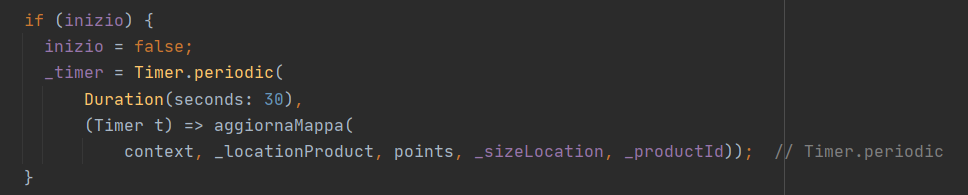
\includegraphics[width=14cm]{immagini/automatico.png}
	\caption{Aggiornamento automatico mappa}
	\label{fig:Aggiornamento automatico mappa}
\end{figure}

\newpage

\subsection{Mappa schermo intero}
Per fare in modo che la mappa fosse più usufruibile dall'utente è stata creata la possibilità di vederla a schermo intero.
Per fare ciò è stato usato un valore booleano, ovvero \textit{ingradisci}, inizialmente uguale a false, che se settato a true permetteva di vedere nello schermo solo la mappa.\\
Cliccando sul bottone \textit{schermo intero} veniva infatti  settato questo valore a true e istantaneamente veniva ricostruita la pagina con la mappa a schermo intero.\\
Una volta che la mappa era a schermo intero, premendo sull'icona con la croce veniva settato il booleano a false ricostruendo sempre la pagina come in precedenza.\\

\begin{figure}[htbp]	
	\centering
	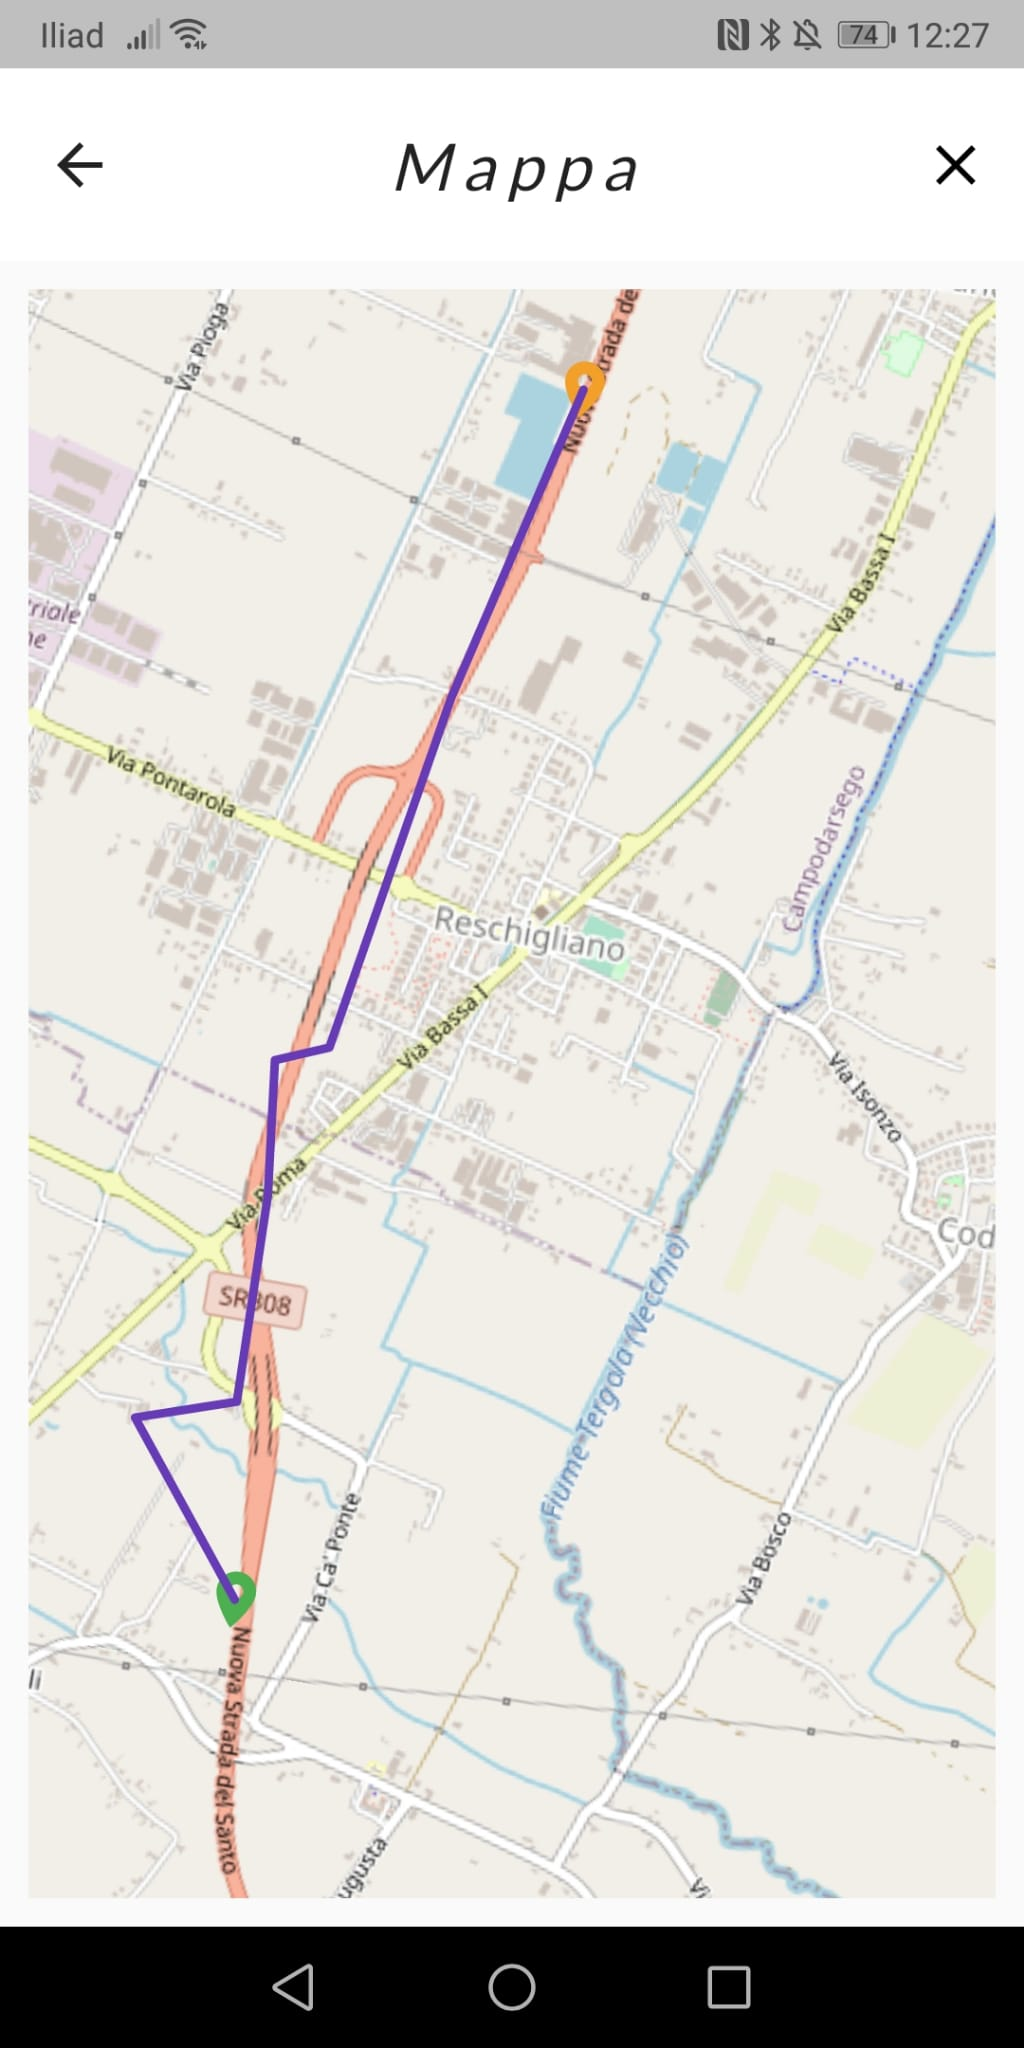
\includegraphics[width=6cm]{immagini/mappaintero.jpeg}
	\caption{Mappa schermo intero}
	\label{fig:Mappa schermo intero}
\end{figure}

\newpage

\subsection{Filtro avanzato di ricerca attività}
Per creare il filtro avanzato è stata creata una funzione \textit{showFilterMenu()} nel file \textit{uscite\_overview\_screen.dart} che contiene una \textit{showDialog}.\\
Per aprire il menù dei filtri bisognerà premere sull'icona dei filtri situata in basso a destra.\\
All'interno di questo menu è possibile filtrare le attività in base allo sport, alla data e se si tratta di tue attività.\\
Per applicare i vari filtri, ovvero quando si preme sull'icona check, è stata utilizzato un booleano che ricostruisce la pagina  con filtro uguale a true e va a chiamare nel provider \textit{uscite.dart} la funzione \textit{findBySporteData} in base ai valori messi nel filtro.\\
L'icona con la croce, una volta premuta, setta il valore del filtro a false e ricostruisce la pagina chiudendo la showdialog dei filtri e cancellando i filtri precedentemente applicati.\\
Per poter capire se abbiamo applicato i filtri basterà guardare se l'icona dei filtri ha il colore verde.\\
Invece se non avremo filtri applicati l'icona avrà il solito colore bianco.\\

\begin{figure}[htbp]	
	\centering
	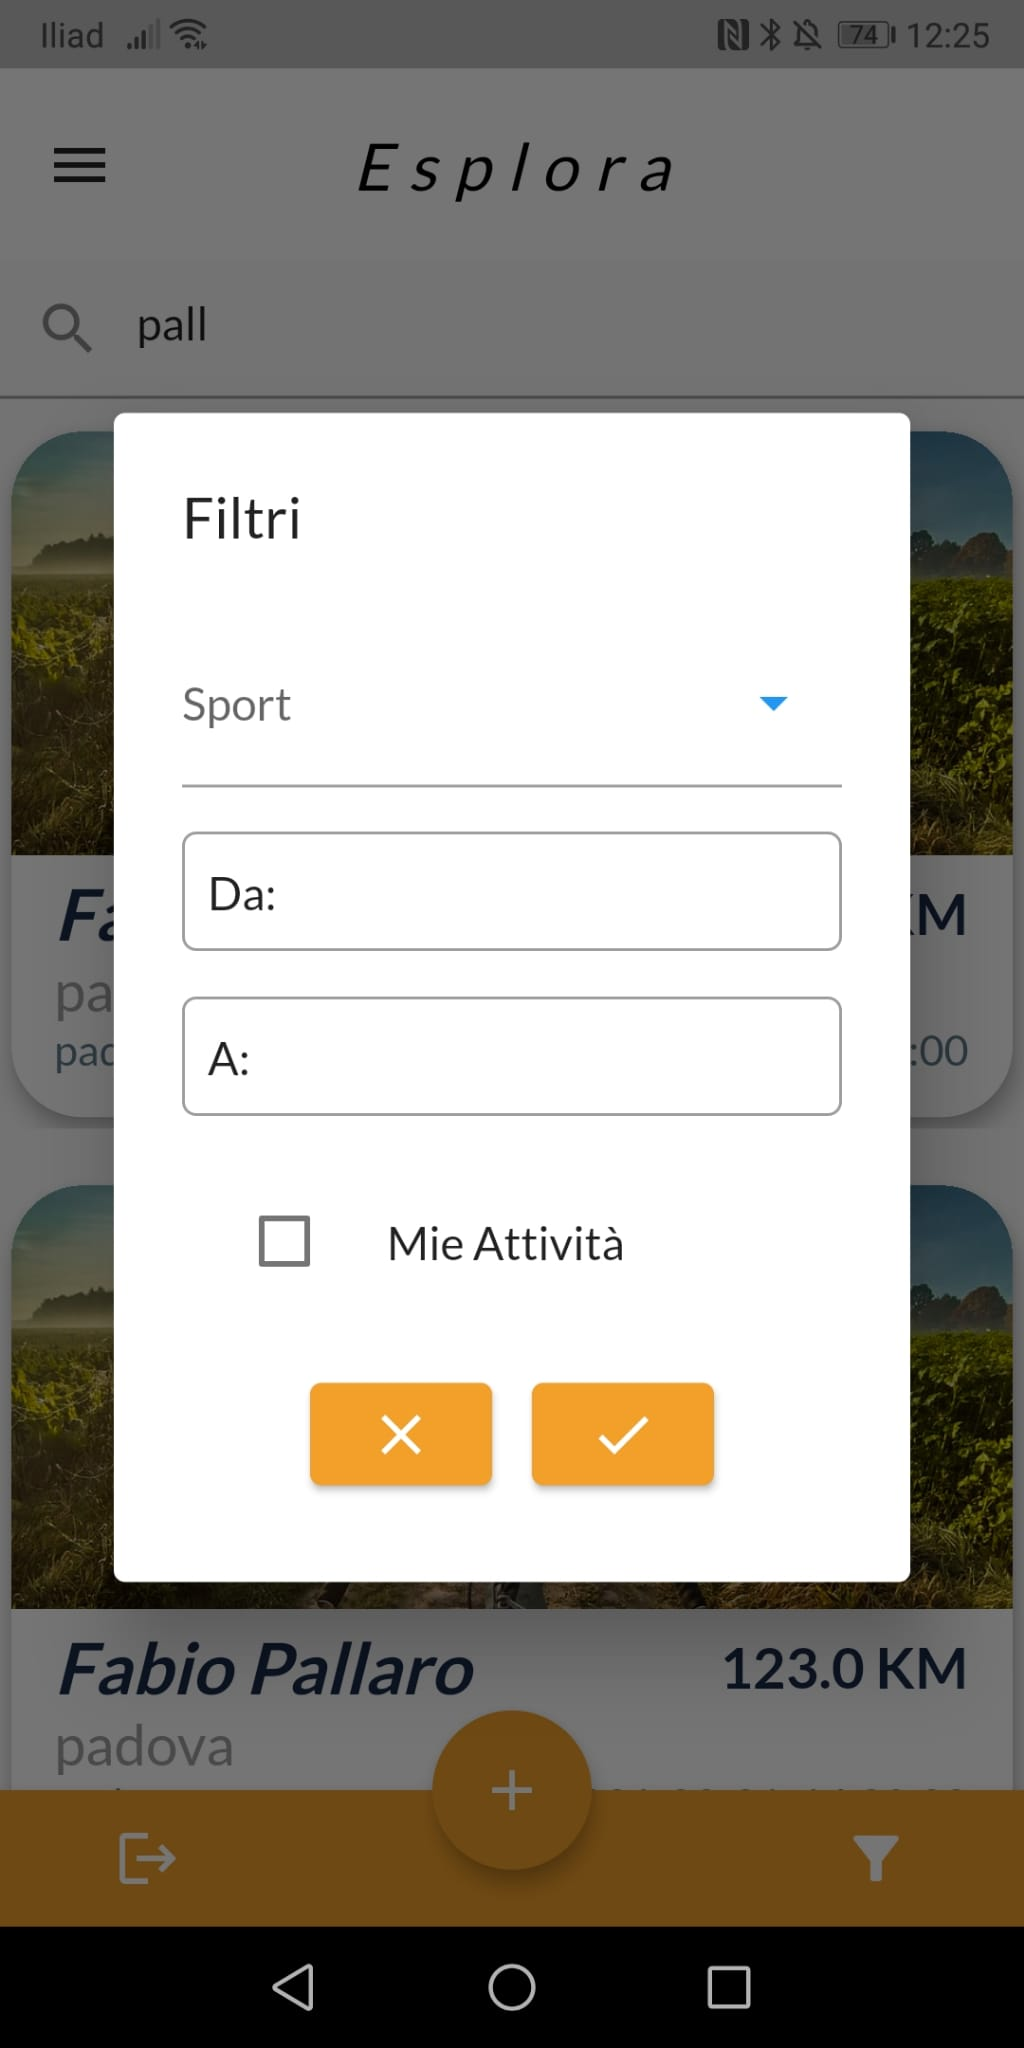
\includegraphics[width=6cm]{immagini/filtroavanzato.jpeg}
	\caption{Filtro avanzato di ricerca attività}
	\label{fig:Filtro avanzato di ricerca attività}
\end{figure}

\newpage

\subsection{Pubblicazione applicazione Play Store}
Questa è l'ultima attività effettuata che non è stata completata ma solo studiata anche se con molte probabilità in futuro è possibile che l'applicazione venga caricata sul Play Store.\\
Per caricare l'applicazione sul Play Store è stata studiata la documentazione fornita da Flutter al seguente indirizzo \url{https://flutter.dev/docs/deployment/android}.
Come prima cosa bisogna lanciare da terminale il seguente comando: \textit{keytool -genkey -v -keystore c:/Users/USER\_NAME/upload-keystore.jks -storetype JKS -keyalg RSA -keysize 2048 -validity 10000 -alias upload}, modificando il percorso.\\
Successivamente dopo aver fatto tutte le configurazioni necessarie bisognerà gestire il file key.properties con i valori appena configurati.\\
Dopo aver apportato le modifiche al file key.properties bisognerà modificare anche il file build.gradle come specificato dalla documentazione.\\
Infine bisognerà, sempre da terminale lanciare il seguente comando: \textit{flutter build appbundle}.\\
Infine per rilasciare l'applicazione bisognerà creare un account al seguente indirizzo \url{https://play.google.com/console/u/0/signup} pagando 25 dollari e successivamente dopo aver superato tutti i test previsti l'applicazione potrà essere rilasciata sul Play Store.\\

\begin{figure}[htbp]	
	\centering
	
\includegraphics[width=8cm]{immagini/playstore.jpg}
	\caption{Play Store}
	\label{fig:Play Store}
\end{figure}

             % Concept Preview
% !TEX encoding = UTF-8
% !TEX TS-program = pdflatex
% !TEX root = ../tesi.tex

%**************************************************************
\chapter{Conclusioni}
\label{cap:conclusioni}
%**************************************************************

\intro{In questo capitolo vengono valutati gli obiettivi raggiunti e infine viene fatta una valutazione personale dello stage svolto.}\\

%**************************************************************
\section{Raggiungimento degli obiettivi}
Nella tabella sottostante vengono rappresentati gli obiettivi raggiunti a fine stage specificando lo stato di completamento di ognuno di essi.\\
\begin{center}
	\begin{table}[h!]
		
		\label{tab:Raggiungimento obiettivi}
		\begin{tabularx}{\textwidth}{|c|p{7cm}|p{2.4cm}|}
			
			\hline
			\textbf{Identificativo} & \centering\textbf{Descrizione} & \textbf{Stato}  \\\hline
			
			O01 & Acquisizione delle competenze sul progetto in generale, il framework Flutter e il linguaggio Dart.  & Completato\\
			\hline
			O02 & Capacità di raggiungere gli obiettivi richiesti in autonomia seguendo il cronoprogramma.  & Completato\\
			\hline	
			O03 & Portare a termine le implementazioni previste con una percentuale di superamento pari all’80\%.  & Completato\\
			\hline
			D01 & Portare a termine le implementazioni previste con una percentuale di superamento pari al 100\%.  & Completato\\
			\hline
			F01 & Realizzazione di una nuova funzionalità per l'app che prevede la gestione Signin con il protcollo Oath2. & Non completato\\
			\hline		
		\end{tabularx}
		\vspace{0.3cm}
		\caption{Raggiungimento obiettivi}
	\end{table}
\end{center}

Si può vedere che in base agli obiettivi stabiliti all'inizio tutti quelli obbligatori e desiderabili sono stati completati.\\
Per quanto riguarda il requisito facoltativo è stato lasciato da parte seppur fosse molto interessante.\\
Il motivo principale di questa scelta è stato presa il fatto che la parte di login era assegnata all'altro stagista e io non l'ho vista con dettaglio.\\
Invece, sempre concordandomi con il tutor Fabio Pallaro, ho optato per concentrarmi su altri aspetti interessanti come la pubblicazione dell'applicazione sul Play Store.


%**************************************************************
\section{Valutazione personale}
Questa esperienza di stage, in sintesi, la posso definire come molto piacevole e importante.\\
Mi ha permesso innanzitutto di entrare a far parte di una nuova realtà come quella del lavoro, in un ambiente molto sano e collaborativo.\\
Sono riuscito a mettere in pratica quanto studiato durante questi tre anni e grazie al lavoro, per lo più autonomo, sono riuscito a individuare i maggiori problemi e a capire come risolverli.\\
Inoltre grazie a questa esperienza ho compreso meglio una nuova tecnologia, abbastanza recente, come Flutter che mi ha fatto appassionare alla programmazione di applicazioni mobile nei vari loro aspetti.\\
In conclusione mi posso ritenere soddisfatto dell'esperienza appena svolta e se in futuro ci saranno altri contatti con l'azienda SyncLab ne sarei profondamente lieto e onorato.


             % Product Prototype           % Conclusioni
\appendix                               
% !TEX encoding = UTF-8
% !TEX TS-program = pdflatex
% !TEX root = ../tesi.tex

%**************************************************************
\chapter{Appendice A}
%**************************************************************

\epigraph{Citazione}{Autore della citazione}



             % Appendice A

%**************************************************************
% Materiale finale
%**************************************************************
\backmatter
\printglossaries
% !TEX encoding = UTF-8
% !TEX TS-program = pdflatex
% !TEX root = ../tesi.tex

%**************************************************************
% Bibliografia
%**************************************************************

\cleardoublepage
\chapter{Bibliografia}

\nocite{*}
% Stampa i riferimenti bibliografici
\printbibliography[heading=subbibliography,title={Riferimenti bibliografici},type=book]

% Stampa i siti web consultati
\printbibliography[heading=subbibliography,title={Siti web consultati},type=online]

1 https://www.synclab.it/
\\
2 https://www.bintmusic.it/uso-smartphone-statistiche-controllo/
\\
3 https://pan-webdesign.it/pages/sviluppo-applicazioni-mobile-possibili-scenari-metodi-applicativi.html
\\
4 http://www.mr-apps.com/it/blog/la-differenza-tra-app-native-app-ibride-e-web-app
\\
5 https://www.icicletech.com/blog/react-native-flutter-ionic-xamarin-nativescript
\\
6 https://dart.dev/
\\
7 https://flutter.dev/
\\
8 https://www.ionos.it/digitalguide/siti-web/programmazione-del-sito-web/cose-flutter/
\\
9 https://nix-united.com/blog/the-pros-and-cons-of-flutter-in-mobile-application-development/\#benefits
\\
10 https://it.wikipedia.org/wiki/Dart\_(linguaggio)\\
\\
11 
https://www.html.it/pag/377313/il-framework-dettagli-tecnici/
\\
12 https://www.html.it/pag/378347/stateful-e-stateless-widget-le-fondamenta-di-unapp-flutter/
\\
13 https://www.geeksforgeeks.org/scaffold-class-in-flutter-with-examples/
\\
14









\end{document}
